% -*- coding: UTF-8 -*-
% hurlex.tex
% hurlex 开发文档

% 我们采用 A4 纸,论文风格
\documentclass[11pt, a4paper]{article}

% 必要的宏包
\usepackage{fontspec, graphicx, titlesec, xunicode, xltxtra, natbib}
\usepackage{indentfirst, listings, xcolor, verbatim, fancyvrb, mdframed}

% 显示中文的名称
\renewcommand{\abstractname}{摘要} 
\renewcommand{\contentsname}{目录} 
\renewcommand{\listfigurename}{插图目录}
\renewcommand{\listtablename}{表格目录}
\renewcommand{\refname}{参考文献}
\renewcommand{\abstractname}{摘要}
\renewcommand{\indexname}{索引}
\renewcommand{\tablename}{表}
\renewcommand{\figurename}{图}
\renewcommand{\lstlistingname}{代码}

% 定义我们的页面样式
\newpagestyle{main}{
	% 字体设置
	\setmainfont{YaHei Consolas Hybrid}

	% 使用中文的断行规则
	\XeTeXlinebreaklocale "zh"
	\XeTeXlinebreakskip = 0pt plus 1pt minus 0.1pt

	% 页边距设置
	\usepackage[top = 1.2in, bottom = 1.2in, left = 1.2in, right = 1in]{geometry}

	% 页眉和页脚设置
	\sethead{\small\S\, \thesection\quad\sectiontitle}{}{$\cdot$~\thepage~$\cdot$}
	\setfoot{}{}{}
	\headrule
	%\footrule

	% 设置章节目录深度
	\setcounter{tocdepth}{1}

	% 设置章节标题格式
	\titleformat{\section}{\centering\Large\bfseries}{\S\,\thesection}{1em}{}
	\titleformat{\subsection}{\large\bfseries}{\S\,\thesubsection}{1em}{}
	
	% 段落首行缩进 2 字符
	\setlength{\parindent}{2em}

	% 段间距
	\setlength{\parskip}{0.5\baselineskip}
}

% 设置文档页的样式
\pagestyle{main}

% 嵌入代码格式设置
\lstset{numbers = left, 
	keywordstyle = \color{blue},
	numberstyle = \small\color{black},
	backgroundcolor = \color{lightgray},
	stepnumber = 1, 
	showspaces = false,
	showtabs = false,
	tabsize = 8,
	breaklines = tr,
	extendedchars = false
}

% 修改日期的显示格式
\renewcommand{\today}{\number\year 年\number\month 月\number\day 日}

% 设置文档标题和作者信息
\title{一个基于x86架构的简单内核实现}
\author{hurley}
\date{\today}

% 设置参考文献的格式
\bibliographystyle{plain}

% 文档内容从这里开始
\begin{document}

% 输出标题
\maketitle

% 摘要
\begin{abstract}
这是一篇阐述如何在基于Intel x86架构的IBM PC机及其兼容计算机上构建一个简单的操作系统内核的教程。\allowbreak
我们将从裸机出发,逐渐展示构建一个简单的操作系统内核的全过程。你可以跟随着笔者的脚步,\allowbreak
慢慢体会一个小内核诞生的整体框架和所有细节,进一步了解操作系统的实现原理和在x86架构上的具体实现。\allowbreak
\end{abstract}

% 换页
\clearpage

% 输出目录
\tableofcontents

% 第1章
% -*- coding: UTF-8 -*-
% hurlex-chapt1.tex
% hurlex 开发文档 第1章内容

\section{项目概述和开发环境配置}

\par 这是一篇阐述如何在基于Intel x86架构的IBM PC机及其兼容计算机上构建一个简单的操作系统内核的教程。\allowbreak
\footnote{这篇教程很大程度上来自《JamesM's kernel development tutorials》这篇文档,感谢原作者的辛勤劳动。\allowbreak
相较而言我的工作在很大的程度上只是转述和查证。}
我们将一起来探索x86CPU的保护模式下操作系统内核的编写方法,一起感受一次完整的探索过程。\allowbreak
虽然这个小内核和一个具有商业价值的操作系统内核相较而言依旧相差甚远。但是通过这样的探索,相信我们能充\allowbreak
分的理解x86保护模式的运行方式和操作系统的基本原理,而这恰恰是传统的通过阅读书籍的方式难以获得的深刻体验。

\par 言归正传,开始我们的征程吧。什么?你已经迫不及待的打开编辑器准备写代码了?别着急,工欲善其事,必先利其器。\allowbreak
我们先来阐述下开发环境和相关的工具配置。

\subsection{选择工作环境}
\par Windows 和 Linux 之争由来已久,我不想在这篇文档里针对这个问题再非口舌。我们的工作环境也选择Linux,\allowbreak
对于Windows用户而言只能说声抱歉了。使用Linux的原因很简单,这里有可以自由使用的一系列的开源\allowbreak
软件能很好的协助我们的开发和调试工作,而在Windows下缺乏相应的免费工具\allowbreak
\footnote {当然也可能是我学习和工作的环境多是Linux,所以对Windows下的工具所知甚少。另外为了避免读者频繁看到诸如\allowbreak
"Windows下如何做,Linux下如何做"的字眼而厌烦,所以就只能牺牲一部分读者的感受了,我在此表示歉意。}
。虽然我的构建环境使用的是Fedora 18,但是这不影响大家对于Linux发行版的选择,因为使用的命令基本上都是相同的的。\allowbreak
\footnote {差异较大的部分应该是软件安装的包管理器了,这个相信大家应该很熟悉自己所使用的发行版所附带的包管理器了。}

\par 同时,为了避免谈及一些Linux基础的命令和基本的计算机概念,我假定读者们已经对以下列出的知识点有一定的理解和掌握:
\begin{itemize}
	\item 熟悉微机原理和基本的操作系统原理,了解基本的计算机原理概念。
	\item 了解和熟悉Intel x86保护模式下的一些名词和概念,至少需要熟悉Intel 8086.
	\item 熟悉和掌握Linux的常用命令,能在Linux下进行基本的系统程序编写。
	\item 掌握简单的x86汇编语言,能读懂和编写简单的汇编程序(至少能看懂)。
	\item 熟练掌握C语言程序的编写,对C语言中较为复杂的语法有所了解。
	\item 理解和掌握C语言程序编译的过程,了解链接的基本原理。
	\item ……
\end{itemize}

\par 我希望之前的描述没有吓到你。也许你本来满怀热情的准备开始干一场"大事业"的热情被一盆水浇凉了很多。假如你没有,\allowbreak
那么我很高兴。即使你真的被那些条款吓到了也不要紧,学习本来就是一个从无到有的过程,操作系统内核的编写本来就是一个\allowbreak
及其复杂和麻烦的过程。尽管我们做的东西甚至只是一个基本原理的演示,但那也是实打实的可以运行在裸机\allowbreak
\footnote{这里的"裸机"指没有安装操作系统的计算机。}
上的小内核。不过千里之行,始于足下。一时的胆怯会在我们逐渐获得的一点点成就感中丧失殆尽。同时我也会尽量降低这个小内核的\allowbreak
难度,给充满热情但相关基础较为薄弱的读者阐述尽可能多的背景资料和原理解析(至少也会给出参考资料的链接)。我相信哪怕\allowbreak
你之前的基础再弱,至少也能"照猫画虎"的构建出一个可以在裸机上运行的小内核。

\par 相信这个体验会对你以后的学习生涯带来很多难以估量的\allowbreak
好处。当你在学习计算机原理的时候,你对计算机的理解将不再是浅浅的浮于表面的概括,而是深刻的掌握了机器运行的基本原理。\allowbreak
那些看似枯燥的理论和概念在你的眼里将是鲜活且富有生机的。相比较一般的用户只是使用计算机而言,我们却在自己的机器上写出\allowbreak
了一个可以运行的操作系统内核。这难道不是一件很酷、很Geek、很好玩的事情吗?

\subsection{选择开发语言}
\par 我们解决了工作环境的问题,接下来是语言的选择了。如果我说是汇编语言的话,恐怕很多读者已经彻底失去了读下去的勇气了。\allowbreak
但是没有办法,有的地方确实需要使用汇编语言去实现。但是聪明的读者已经注意到前文提到了C语言,没错,很大程度\allowbreak
上的代码使用C语言来实现。所以不用过于担心,这个项目不会太难的。

\subsection{选择开发工具}
\par 接着是选择开发使用的工具了,这个我简单的列出来吧。首先C语言的编译器肯定使用gcc,链接器自然也就是ld了。同时大项目\allowbreak
自然也少不了GNU make这个构建工具了。至于汇编编译器我们选择nasm这个开源免费的编译器,以便使用大多数读者习惯的Intel\allowbreak
风格的汇编语法。不过考虑到需要在一些C语言代码中内联汇编指令,而gcc使用的是AT\&T风格的汇编语法,所以大家还是需要\allowbreak
掌握一部分的AT\&T风格的语法的。不过这个倒不必担心,随意Google一下就有好多的资料可以学习。这些就是开发使用的多数\allowbreak
工具了,其他的工具我会在使用的时候再介绍。

\par 现在看起来一切都还好不是吗?等等,我们写用户级别程序自然可以直接运行,可现在是要写一个操作系统内核啊。\allowbreak
我们在哪里运行它?难道再需要一台计算机吗?当然不用了,我们可以使用虚拟机。如果你使用过相关的虚拟机软件,比如Vmware\allowbreak
或者Virtual Box之类的话那就太好了。当然没用过也不必担心,其实虚拟机就是一个软件。它可以在宿主机上\allowbreak
\footnote{运行这个虚拟机软件的计算机叫做宿主机}模拟出一个虚拟的硬件环境再次运行一个操作系统,而且运行的操作系统\allowbreak
重启和关机都是虚拟的,不需要重启宿主机。而且虚拟机里运行的程序不会对宿主机造成影响\allowbreak
\footnote{至少我还从来没见过可以穿透虚拟机而损坏到宿主机的程序,而且以我目前的水平肯定写不出来,大家尽管放心。:) }
,所以大家可以放心的编写代码而不必担心对自己的机器造成损坏。

\par 不过我们这次使用的不是大多数读者熟悉的Vmware或者Virtual Box,而是一款叫做qemu\allowbreak
的虚拟机。为什么呢?因为有调试的需要。我们需要一个能调试其上运行着的操作系统的虚拟机,而qemu是个不错的选择。\allowbreak
也许你听过另一款叫做bochs的虚拟机也支持调试,但这次不选择bochs。因为各大Linux发行版软件源里的bochs默认是不带有\allowbreak
功能的,所以需要重新下载源码编译。而从源里安装的qemu通常直接可以和gdb进行联合调试,所以很省事。而且大家作为一个linuxer,\allowbreak
对gdb的使用也不需要我多费唇舌吧?我本着易用简单的理念开始写这篇文档,倘若在环境配置上就让大家感到无所适从的话就不好了。\allowbreak
如果你熟悉bochs,那自然也可以使用,我会在本章节的末尾给出一个bochs的配置以供有需要的读者参考。

qemu 的安装方法很简单,以Fedora为例,只需执行以下命令即可。
\begin{Verbatim}[frame=single]
    sudo yum install qemu -y
\end{Verbatim}

\par Ubuntu 之类的debian系列的发行版是以下命令:
\begin{Verbatim}[frame=single]
    sudo apt-get install qemu
\end{Verbatim}

\par 不过安装完成后需要建立一个符号链接文件,命令如下:

\begin{Verbatim}[frame=single]
    sudo ln -s /usr/bin/qemu-system-i386 /usr/bin/qemu
\end{Verbatim}

\par 大家可以根据自己实际的软件安装目录去配置。

\subsection{开发中用到的脚本文件}

\subsubsection{Makefile}
\par 首先是编译时使用的Makefile。需要强调的是,这个Makefile在我们整个项目的进程中\allowbreak
几乎不会被修改。所以学会它就等于学会了整个内核项目的编译方式,很划算哦。
\footnote{可能有的地方你不是很理解,那么你可以试着去Google上搜索你不理解的关键字,\allowbreak
也可以参考Makefile或者gcc的手册,这些在网上都很容易检索到。}
\footnote{这个Makefile很简单而且颇具启发意义。只要简单修改一些参数就可以在其他项目里使用了。}

\begin{lstlisting}[language = sh, caption = Makefile]
#!Makefile

C_SOURCES = $(shell find . -name "*.c")
C_OBJECTS = $(patsubst %.c, %.o, $(C_SOURCES))
S_SOURCES = $(shell find . -name "*.s")
S_OBJECTS = $(patsubst %.s, %.o, $(S_SOURCES))

CC = gcc
LD = ld
ASM = nasm

C_FLAGS = -c -Wall -m32 -ggdb -gstabs+ -nostdinc -fno-builtin -fno-stack-protector -I include
LD_FLAGS = -T tools/kernel.ld -m elf_i386 -nostblib
ASM_FLAGS = -f elf -g -F stabs

all: $(S_OBJECTS) $(C_OBJECTS) link update_image

.c.o:
	@echo 编译代码文件 $< ...
	$(CC) $(C_FLAGS) $< -o $@

.s.o:
	@echo 编译汇编文件 $< ...
	$(ASM) $(ASM_FLAGS) $<

link:
	@echo 链接内核文件...
	$(LD) $(LD_FLAGS) $(S_OBJECTS) $(C_OBJECTS) -o hx_kernel

.PHONY:clean
clean:
	$(RM) $(S_OBJECTS) $(C_OBJECTS) hx_kernel

.PHONY:update_image
update_image:
	sudo mount floppy.img /mnt/kernel
	sudo cp hx_kernel /mnt/kernel/hx_kernel
	sleep 1
	sudo umount /mnt/kernel

.PHONY:mount_image
mount_image:
	sudo mount floppy.img /mnt/kernel

.PHONY:umount_image
umount_image:
	sudo umount /mnt/kernel

.PHONY:qemu
qemu:
	qemu -fda floppy.img -boot a

.PHONY:bochs
bochs:
	bochs -f tools/bochsrc.txt

.PHONY:debug
debug:
	qemu -S -s -fda floppy.img -boot a &
	sleep 1
	cgdb -x tools/gdbinit

\end{lstlisting} 

\subsubsection{kernel.ld}
\par 接下来是项目初步采用的链接器脚本的定义。

\begin{lstlisting}[caption = script/kernel.ld]
/*
 *      kernel.ld -- 针对 kernel 格式所写的链接脚本
 */

ENTRY(start)
SECTIONS
{
	/* 段起始位置 */

	. = 0x100000;
	.text :
	{
		*(.text)
		. = ALIGN(4096);
	}

	.data :
	{
		*(.data)
		*(.rodata)
		. = ALIGN(4096);
	}

	.bss :
	{
		*(.bss)
		. = ALIGN(4096);
	}

	.stab :
	{
		*(.stab)
		. = ALIGN(4096);
	}
	
	.stabstr :
	{
		*(.stabstr)
	 	. = ALIGN(4096);
	}

	/DISCARD/ : { *(.comment) *(.eh_frame) }
}
\end{lstlisting}
 
\par 这个脚本告诉ld程序如何构造我们所需的内核映像文件。

\par 首先,脚本声明了内核程序的入口地址是符号 "start" 。然后声明了段起始位置0x100000(1MB),接着是第一个段.text段(代码段)\allowbreak
、已初始化数据段.data、未初始化数据段.bss以及它们采用的4096的页对齐方式。Linux GCC 增加了额外的数据段.rodata,这是一个\allowbreak
只读的已初始化数据段,放置常量什么的。另外为了简单起见,我们把.rodata段和.data段放在了一起。最后的stab和stabstr段暂时无\allowbreak
需关注,等到后面讲到调试信息的时候就会明白。

\par 如果你对这里的ld链接器的脚本不是很理解也不是很重要,只要理解了脚本表示的意思就好。
\footnote{如果你对编译和链接的过程所知甚少的话,那么我厚脸推荐你我的博客看两篇文章。分别是\allowbreak
《编译和链接的那些事》(上/下) 地址是:http://toqianmo.sinaapp.com/?p=323 和 \allowbreak
http://toqianmo.sinaapp.com/?p=357}
\footnote{如果你对进程的地址空间不是很熟悉的话,建议你先去Google上检索相关的资料,我的博客也有一篇讲解\allowbreak
Linux下进程的线性地址空间的文章可以供你参考,地址是:http://toqianmo.sinaapp.com/?p=397}

\par 我们所用到的脚本暂时就是这两个,随着项目的逐渐展开,还会有陆续的代码加进来。

\par 我目前的目录结构是这样的:
\begin{Verbatim}[frame=single]
.
|-- Makefile
`-- scripts
    `-- kernel.ld

1 directory, 2 files
\end{Verbatim}
\par 你也可以按照这个目录来放置代码,这样会比较清晰。至于项目名称,既然是我们自己写,那就由我们自己随意取名啦。
\footnote{我的小内核叫做hulex。大家可以给自己写的内核自由命名,做一个属于自己的操作系统内核。}

\subsubsection{bochs 虚拟机的配置文件}
\par 我遵守承诺,给bochs的读者提供一份bochs的配置参考。其实熟悉bochs的读者估计都比我写的好,根本用不到我这个班门弄斧的配置。
\footnote{使用qemu的用户是不是很疑惑,怎么没有qemu虚拟机的配置文件呢?嘿嘿,仔细读Makefile,它已经包含\allowbreak
在Makefile里了,也就是几个命令行参数,简单吧?}

\begin{lstlisting}[caption = Bochs 的配置文件]
# ------------------------------------------------------------
# Bochs 配置文件
#
# ------------------------------------------------------------

# 开始 gdb 联合调试,这很重要
gdbstub: enabled=1,port=1234,text_base=0,data_base=0,bss_base=0

# 内存
megs: 32

# ROM 文件
romimage: file="$BXSHARE/BIOS-bochs-latest"
vgaromimage: file="$BXSHARE/VGABIOS-lgpl-latest"

# 软盘
floppya: 1_44=floppy.img, status=inserted
boot: a

# 启动设备为软盘
boot: floppy

# 鼠标 不启用
mouse: enabled=0

# 键盘 启用 US 键盘映射
keyboard_mapping: enabled=1, map="$BXSHARE/keymaps/x11-pc-us.map"

# CPU 配置
clock: sync=realtime
cpu: ips=1000000
\end{lstlisting}

\par 这里要注意的是:一般来说各大Linux发行版软件源里自带的bochs没有开启gdb的联合调试功能。这就需要我们自己下载\allowbreak
源代码编译,具体的方式请有需要的读者自行上网检索。不过我还是推荐使用qemu,毕竟没有人会和简单过不去,不是吗?

% 第2章
% -*- coding: UTF-8 -*-
% hurlex-chapt2.tex
% hurlex 开发文档 第2章内容

\section {计算机启动、GRUB 以及 multiboot 标准}

\par GRUB的全称是GRand Unified Bootloader,是一个多重操作系统启动管理器,用来引导不同的操作系统。\allowbreak
Linuxer和喜欢折腾多系统的读者们想必对GRUB并不陌生吧?但是在详细描述GRUB之前,我们得先来简述一下操作系统的启动过程。\allowbreak
本着别人写过的我们就不写的原则,笔者推荐来自阮一峰博客的一篇文章给大家《计算机是如何启动的?》。
\footnote{地址在 http://www.ruanyifeng.com/blog/2013/02/booting.html}

\par 看过这篇文章之后,想必大家已经在宏观上对计算机的启动过程有了初步的了解。接下来我们细化这个过程,并且着重阐述\allowbreak
其中和我们的项目相关的内容。一直没有说明的是,我们的目标内核是32位的。因为我们只是原理学习,64位繁杂的细节会使得\allowbreak
整个项目难度加大,这是笔者不愿意看到的。
\footnote{其实你可以理解为笔者压根就不懂64位,所以不敢过多谈论。}

\par 我们先来一起复习计算机原理之类的课程中对于CPU寻址的一些概念吧。首先,我们的内核使用32位的地址总线来寻址,\allowbreak
所以我们能编址出2的32次方,也就是4G的地址空间。那么我们的第一个问题是,这4G的空间指向哪里?我想大多数读者的第一反应\allowbreak
都是内存吧?我们知道在主板上除了内存还有BIOS、显卡、声卡、网卡\footnote{这里就原谅笔者使用这些不专业的词汇吧。}\allowbreak
等外部设备,CPU需要和这些外设进行通信。那么实现通信自然就得有地址,不然怎么表示数据的去向呢?比如显卡内部就有自己的一些存储单元\allowbreak
\footnote{甚至还有独立的GPU,我们这个简单的内核不用关注这个。}。在x86下,我们通过端口读写的方式控制这些外部存储单元,\allowbreak
当我们需要访问这些存储单元的时候,就需要给予一个访问地址来区分每一个读写单元。

\par 说到这里,我们需要引出两个专业名词:端口统一编址和端口独立编址。还记得我们刚说的4G地址空间吗?所谓的\allowbreak
端口统一编址就是把所有和外设存储单元对应的端口直接编址在这4G的地址空间里,当我们对某一个地址进行访问的时候实际上\allowbreak
是在访问某个外设的存储单元。而端口独立编址就是说这些端口没有编址在地址空间里,而是另行独立编址。\allowbreak
而x86架构部分的采用了端口独立编址,又部分的采用了端口统一编址。部分外设的部分存储单元直接可以通过某个内存地址访问,\allowbreak
而其他部分在一个独立的端口地址空间中,需要使用in/out指令去访问,我们用到的时候再来细说。

\par 上文简单的介绍了一下地址空间的概念,我们接下来详细分析CPU在加电后的启动过程。这里可能比较枯燥和难以理解,但是没关系,\allowbreak
这里的流程是固化的,程序员们能做的很有限。\footnote{当然了,设计BIOS的程序员可以在这里大显身手。}\allowbreak
笔者增加这一章只是为了读者们能够充分理解我们之后内容的原理,并没有和编程相关的东西,所以只要大致理解就好。

\par 我们从按下电源开始。首先是CPU重置。主板加电之后在电压尚未稳定之前,主板上的北桥控制芯片会向CPU发出重置信号(Reset),\allowbreak
此时CPU进行初始化。当电压稳定后,控制芯片会撤销Reset信号,CPU便开始了模式化的工作。此时形成的第一条指令的地址是0xFFFFFFF0\allowbreak
\footnote{对这个地址有疑问的话,请参考《Intel IA-32 Intel Architecture Software Developer’s Manual Volume 3:System \allowbreak
Programming Guide Section》的9.1.4 章节。或者参考笔者博客的一篇文章《基于Intel 80×86CPU的IBM PC及其兼容计算机的启动流程》\allowbreak
,地址是:http://toqianmo.sinaapp.com/?p=310 P.S. 古老的8086处理器是0xFFFF0这个地址。}\allowbreak
,从这里开始,CPU就进入了一个"取指令-翻译指令-执行"的循环了。所以我们需要做的就是在各个阶段提供给CPU相关的数据,\allowbreak
以完成这个"接力赛"。这个接力过程中任何一个环节如果出现致命问题,其导致的直接后果就是宕机。死机是最好的结果,\allowbreak
最坏的结果是程序在"默默的"破坏我们的数据,所以一定要谨慎对待。

\par 那么,这个地址指向哪呢?大家一定想到了,它指向BIOS芯片里。我们刚刚说过,在4G的地址空间里,有一些地址是分给外设的,\allowbreak
这个地址便是映射到BIOS的。我们知道,计算机刚加电的时候内存等芯片尚未初始化,所以也只能是指向BIOS芯片里已经被"固化"的指令了。\allowbreak

\par 紧接着就是BIOS的POST(Power On Self Test,上电自检)过程了,BIOS对计算机各个部件开始初始化,如果有错误会给出报警音。\allowbreak
当BIOS完成这些工作之后,它的任务就是在外部存储设备中寻找操作系统,而我们最常用的外存自然就是硬盘了。自己安装过操作系统的\allowbreak
读者应该都设置过BIOS选项吧?BIOS里面就有一张启动设备表\footnote{其实严格的说,数据保存在CMOS芯片里,BIOS存放的是程序代码。},\allowbreak
BIOS会按照这个表里面列出的顺序查找可启动设备。那么怎么知道该设备是否可以启动呢?规则其实很简单:如果这个存储设备的第一个扇区\allowbreak
中512个字节\footnote{不见得所有设备的扇区都是512字节,这篇文档我们只针对PC机而言,以后不再注释。}\allowbreak
的最后两个字节是0x55和0xAA,那么该存储设备就是可启动的。这是一个约定,所以BIOS会对这个列表中的设备逐一检测,只要有一个设备满足\allowbreak
要求,后续的设备将不再测试。

\par 当BIOS找到可启动的设备后,便将该设备的第一个扇区加载到内存的0x7C00处,并且跳转过去执行。而我们要做的事情,便是从构造\allowbreak
这个可启动的扇区开始。

\par 因为一个扇区只有512字节,放不下太多的代码,所以常规的做法便是在这里写下载入操作系统内核的代码\footnote{或者载入另一段\allowbreak
代码,这段代码负责查找和载入内核。},这段代码就是所谓的bootloader程序。一般意义上的bootloader负责将软硬件的环境设置到一个\allowbreak
合适的状态,然后加载操作系统内核并且移交执行权限。而GRUB是一个来自GNU项目的多操作系统启动程序。它是多启动规范的实现,\allowbreak
允许用户可以在计算机内同时拥有多个操作系统,并在计算机启动时选择希望运行的操作系统。

\par 引出GRUB的原因很简单:笔者不准备自己实现bootloader程序。理由有二:其一,实现bootloader牵扯太多我们在后期才要讲述的\allowbreak
知识。我们与其前期简陋的实现这个bootloader,还不如就用现成的优秀实现,以后有机会自己再学着改进;第二,笔者想在后面把这个小\allowbreak
安装到物理机器上去,而读者们相比在自己的机器上已经有了多个操作系统了。这样的话如果我们非得实现自己的bootloader的话,\allowbreak
势必会造成和已有操作系统的不兼容。所以,笔者干脆决定直接使用GRUB来加载我们的小内核。以后我们就能让它很简单的安装在我们的\allowbreak
物理机器上,这样的话我们能拥有一个Linux系统和我们自己小内核共存的计算机了。如果你愿意的话,也可以再加上一个Windows系统。

\par 听起来很不错吧?那么问题是我们怎么能让GRUB加载我们的小内核呢?答案是GRUB提供的multiboot规范。这份规范是描述如何\allowbreak
构造出一个能够被GRUB识别,并且按照我们定义的规则去加载的操作系统内核。目的很明确吧?具体的协议在网上很容易检索到,\allowbreak
也有不少中文版本的翻译,所以笔者不再详细解释这个协议。希望对这个协议陌生的读者们先去网上得到一份具体的说明,\allowbreak
仔细的阅读一遍后再阅读下一章节。在下一章节中,我们将自己动手构建出一个可以运行的"Hello, kernel OS"程序,拭目以待吧。


% 第3章
% -*- coding: UTF-8 -*-
% hurlex-chapt3.tex
% hurlex 开发文档 第3章内容

\section{裸机上运行的 Hello OS Kernel}

\par 不知道前两章的文字大家看烦了没有?除了第一章还有简单的动手任务之外,之后都是无聊的文字描述了。嘿嘿,必要的铺垫还是得有的,\allowbreak
虽然以后大段的概念依然少不了,但是从本章开始,我们就要开始进入实战阶段了。

\subsection{Makefile和ld脚本的简单解释}

\par 我们先简单的解释一下之前的Makefile和ld链接脚本的一些字段,如果你已经掌握了,那大致浏览下就可以跳过这段文字了。

\par 先来看Makefile中关于gcc编译参数的这一行:

\begin{Verbatim}[frame=single]
  C_FLAGS = -c -Wall -m32 -ggdb -gstabs+ -nostdinc -fno-builtin
		-fno-stack-protector -I include
\end{Verbatim}

\par 我们只解释以下重要的几个参数:
\begin{itemize}
	\item -m32 是生成32位代码,这样的话我们的开发环境也可以使用64位的Linux系统。
	\item -ggdb 和-gstabs+ 是添加相关的调试信息,调试对后期的排错很重要。
	\item -nostdinc 是不包含C语言的标准库里的头文件。\allowbreak
		\footnote{尽管可以使用C语言进行开发,但是几乎所有C语言的库函数和我们告别了。因为那些库函数都是在特\allowbreak
		定操作系统平台之上的实现,而我们要做的正是实现这样一个平台,所以想用C语言库的话就需要自己实现了。}
	\item -fno-builtin 是要求gcc不主动使用自己的内建函数,除非显式声明。
		\footnote{gcc有很多内建函数用来替换一些C语言的库函数以提升效率,比如把只有一个字符串参数的printf函数替换为puts函数。}
	\item -fno-stack-protector 是不使用栈保护等检测。
\end{itemize}

\par 接着是ld链接命令的参数:
\begin{Verbatim}[frame=single]
  LD_FLAGS = -T scripts/kernel.ld -m elf_i386 -nostblib
\end{Verbatim}

\begin{itemize}
	\item -T scripts/kernel.ld 是使用我们自己的链接器脚本。
	\item -m elf\_i386 是生成i386平台下的ELF格式的可执行文件,这是Linux下的可执行文件格式。
	\item -nostdlib 是不链接C语言的标准库,原因上文已经交代过了。
\end{itemize}

\par 接下来讨论链接器脚本。

\par 我们知道一个可执行的文件大致由代码段和数据段组成,但是操作系统怎么正确加载它呢?事实上可执行文件有义务向操作系统提供\allowbreak
代码段和数据段位置等信息,以便操作系统正确找到它的代码段和数据段并加载执行。通常这个信息被统一组织放置在可执行文件的头部区域。\allowbreak
不同的操作系统中自然就设计了不同的组织方式,比如Linux常见的ELF(Executable and Linkable Format,可执行链接格式)格式,\allowbreak
windows下常见的PE(Portable Executable,可移植的可执行文件)格式都是。\allowbreak
\footnote{其实Linux下的ELF格式和Windows下的PE格式都是COFF(Common Object File Format,通用对象文件格式)\allowbreak
格式的一个变种。}而ld支持很多种链接格式,我们可以在参数里指定。那为何选择ELF格式呢?原因很简单,因为GRUB可以检测\allowbreak
识别出ELF格式的可执行文件,并且能找到相关的代码段和数据段的位置信息,从而正确的把我们的内核加载到正确的位置上去。

\par 看懂了这个Makefile和链接器脚本,我们就向成功迈出了一大步了。大家还记得上一章谈过的GRUB Multiboot标准吗?\allowbreak
只要按照标准生成规范的Multiboot引导信息,同时使用标准的ELF格式,GRUB就能把我们的内核正确的加载和执行了。

\par 说了这么多,现在大家对计算机从加电到执行我们的内核的过程有概念了吧?如果感觉还是很模糊也不要紧,毕竟第一次接触\allowbreak
这些东西难免需要时间消化。随着我们研究的展开,相信你会越来越清晰的。\allowbreak
\footnote{不知道我在前面说的编译链接的过程和可执行文件的结果大家了解过没?没有的话请回去看明白了再回来。因为这直接\allowbreak
关系到你对后续章节的理解程度。如果上面的描述你看的是稀里糊涂的话,还请你先学习了相关的知识背景之后再继续和我做下去,\allowbreak
否则稀里糊涂的玩下去意义真的不是很大,毕竟这不是用来应付的家庭作业。}

\subsection{启动镜像的制作}

\par 解决了理论上的问题之后,我们来解决一个现实的问题。这个问题是,这个小内核放在哪里?虚拟机是它运行的场所,那么虚拟\allowbreak
磁盘自然就是安放内核的选择了。不过我们这次不选择硬盘,而是选择已经几乎消失殆尽的1.44MB的软盘。为什么?说实话是因为比较简单。\allowbreak
\footnote{这个答案有点囧是不是?其实从一开始到现在,我们已经为了求简做了很多妥协了,从精简的描述到通俗的概念解释,再到使用\allowbreak
现成的bootloader程序,现在又使用简单的外部存储。这么做一是我自己确实水平很有限,二是这篇文档的定位是初学者,不能过于复杂\allowbreak
,所以还请大家多多担待。}

\par 在Linux下制作一个1.44MB软盘的技术太简单了,甚至dd命令也可以做一个出来。\allowbreak
\footnote{老规矩,大家自己上Google搜索,学会自己探索是很重要的。}不过在这个软盘镜像上安装一个GRUB稍有难度,\allowbreak
所以大家直接可以使用我提供的已经安装好了GRUB的软盘镜像。\allowbreak
\footnote{这个软盘镜像的作者是Jamesm先生,再次表示感谢。不过建议有基础的读者去Google检索相关资料,自己做一个出来。}

\par 大家准备好镜像了吗?OK!万事俱备,只欠代码了。让我们开始最激动人心的探索吧!
\par 抱歉,我又得打断一下。因为必须引入一个新的术语名词——文件系统。什么是文件系统呢?其实简单的说,这里所谓\allowbreak
的文件系统指的是操作系统用于明确磁盘或分区上的文件存储的方法和数据结构,即在磁盘上组织文件的方法。如果把这个1.44MB\allowbreak
的软盘可以看做一个巨大的数组,那么每个数组成员都是一个扇区,拥有512字节的存储单元。现在需要往这个软盘上写入文件,那么自然\allowbreak
需要一套合适的管理规则,否则的话岂不是全乱套了?就和这篇文档一样,不同的章节被划分在不同的位置,同时在最前面有所有章节\allowbreak
的目录,这就是一种对信息的组织方式,文件系统也不过是这么一套组织策略罢了。\allowbreak
\footnote{当然,这里只是通俗的解释了文件系统的基本概念,其实设计一个优秀的文件系统是一件并不容易的事情,需要考虑到很多因素。}

\par 考虑到兼容因素,自然是选择目前使用的比较广泛的文件系统了,这样的话也便于我们对软盘里面存储的文件进行管理操作。\allowbreak
\footnote{这个理由听起来不错。其实弱弱的说一句,还有一个原因是我自己目前没有设计一个文件系统的能力。嘘~这是秘密,\allowbreak
千万别说出去。}那么使用什么文件系统呢?软盘一般使用的是FAT12文件系统,所以我们也就不标新立异了。这个文件系统也很\allowbreak
简单,后期大家有兴趣的话甚至可以在我们的内核里实现能处理这个文件系统的代码。至于FAT12文件系统的资料也很多,我就不详细说了。\allowbreak
\footnote{经过前面的几次去Google检索,相信大家现在搜索资料的水平强了不少吧?那就再接再厉,自己简单浏览下FAT12的一些资料吧。}\allowbreak
GRUB支持从很多常见的文件系统中去读取和载入内核文件,当然也包括我们使用的FAT12格式。我们在自己开发使用的Linux系统上很容易就\allowbreak
可以挂载和读写这个虚拟软盘里的文件,这给开发带来了极大的便利。我们经常做的事就是拷贝编译好的内核进去,然后在虚拟机\allowbreak
运行。另外这个虚拟软盘文件里还有GRUB和它的配置文件,我提供的软盘镜像里安装的是一个很早的GRUB版本,它的配置文件简单到\allowbreak
一看就懂。\footnote{本着够用就好的原则,较早的GRU版本就完全满足我们的需求了,而新版的GRUB配置起来比较麻烦。}\allowbreak
所以大家完全可以自己看着修改。\footnote{其实也没有什么需要改的,主要是GRUB载入的内核文件名。我的内核名叫做hx\_kernel,\allowbreak
如果你嫌麻烦,和我叫一个名字就不用修改GRUB配置了。}

\subsection{内核的入口和初始化}

\par 前期的铺垫到这里就告一段落了,下面我们开始编码工作吧。

\par 代码从什么函数开始执行呢?如果你记忆力足够好的话你会记得ld链接脚本里面的一行文字:

\begin{Verbatim}[frame=single]
  ENTRY(start)
\end{Verbatim}

\par 这就意味着我们告诉了ld链接器入口函数是start,所以代码从start函数开始。\allowbreak
\footnote{入口可以自由定义,只要在ld链接脚本里修改就可以。要知道我们现在是在写一个操作系统内核,在这里我们几乎可以定制一切。}

\par 大家先来一起围观下入口部分的代码全貌:

\begin{lstlisting}[language = {[x86masm]Assembler}, caption = boot/boot.s]
; ----------------------------------------------------------------
;
; 	boot.s -- 内核从这里开始
;
; ----------------------------------------------------------------

; Multiboot 魔数,由规范决定的
MBOOT_HEADER_MAGIC 	equ 	0x1BADB002

; 0 号位表示所有的引导模块将按页(4KB)边界对齐
MBOOT_PAGE_ALIGN 	equ 	1 << 0

; 1 号位通过 Multiboot 信息结构的 mem_* 域包括可用内存的信息
; (告诉GRUB把内存空间的信息包含在Multiboot信息结构中)
MBOOT_MEM_INFO 		equ 	1 << 1    

; 定义我们使用的 Multiboot 的标记
MBOOT_HEADER_FLAGS 	equ 	MBOOT_PAGE_ALIGN | MBOOT_MEM_INFO

; 域checksum是一个32位的无符号值,当与其他的magic域(也就是magic和flags)
; 相加时,要求其结果必须是32位的无符号值 0 (即magic+flags+checksum = 0)
MBOOT_CHECKSUM 		equ 	-(MBOOT_HEADER_MAGIC+MBOOT_HEADER_FLAGS)

; 符合Multiboot规范的 OS 映象需要这样一个 magic Multiboot 头
; Multiboot 头的分布必须如下表所示:
; ----------------------------------------------------------
; 偏移量  类型  域名        备注
;
;   0     u32   magic       必需
;   4     u32   flags       必需 
;   8     u32   checksum    必需 
;
; 我们只使用到这些就够了,更多的详细说明请参阅 GNU 相关文档
;-----------------------------------------------------------

;-----------------------------------------------------------------------------

[BITS 32]  	; 所有代码以 32-bit 的方式编译
section .text 	; 代码段从这里开始

; 在代码段的起始位置设置符合 Multiboot 规范的标记

dd MBOOT_HEADER_MAGIC 	; GRUB 会通过这个魔数判断该映像是否支持
dd MBOOT_HEADER_FLAGS   ; GRUB 的一些加载时选项,其详细注释在定义处
dd MBOOT_CHECKSUM       ; 检测数值,其含义在定义处

[GLOBAL start] 		; 向外部声明内核代码入口,此处提供该声明给链接器
[GLOBAL glb_mboot_ptr] 	; 向外部声明 struct multiboot * 变量
[EXTERN kern_entry] 	; 声明内核 C 代码的入口函数

start:
	cli  			 ; 此时还没有设置好保护模式的中断处理,要关闭中断
				 ; 所以必须关闭中断
	mov esp, STACK_TOP  	 ; 设置内核栈地址
	mov ebp, 0 		 ; 帧指针修改为 0
	and esp, 0FFFFFFF0H	 ; 栈地址按照16字节对齐
	mov [glb_mboot_ptr], ebx ; 将 ebx 中存储的指针存入全局变量
	call kern_entry		 ; 调用内核入口函数
stop:
	hlt 			 ; 停机指令,可以降低 CPU 功耗
	jmp stop 		 ; 到这里结束,关机什么的后面再说

;-----------------------------------------------------------------------------

section .bss 			 ; 未初始化的数据段从这里开始
stack:
	resb 32768 	 	 ; 这里作为内核栈
glb_mboot_ptr: 			 ; 全局的 multiboot 结构体指针
	resb 4

STACK_TOP equ $-stack-1 	 ; 内核栈顶,$ 符指代是当前地址

;-----------------------------------------------------------------------------
\end{lstlisting} 

\par 我们简单的介绍下这段代码做的事情。
\par 首先是一些宏定义,定义了Multiboot标准的魔数和几个标识,GRUB会读取这些信息以判断我们的意图。真正的代码是从\allowbreak
39行以后开始的,首先我们在代码段的入口位置之前定义了几个Multiboot规范要求的配置信息,其实也就是3个4字节变量。我们通过\allowbreak
这几个变量告诉了GRUB我们要求它提供可用内存的信息,而且要求内核中所有的段在内存里按照4KB进行对齐。\allowbreak
\footnote{后面谈到分页后你就明白这里的4KB对齐之类的含义了,暂时先按照我的要求做吧。}紧接着就是我们内核的入口函数\allowbreak
start了,入口代码很短,主要做的是关闭中断,传参数(按照协议,GRUB把一些计算机硬件和我们内核文件相关的信息放在了一个结构体\allowbreak
中,并且将这个结构体指针放在了ebx寄存器中)并且调用内核的入口函数。\footnote{如果你对这里不是很清楚的话,暂时就先跳过去,到后面\allowbreak
解释完函数调用栈之后再回来看。如果你现在非要现在弄明白的话,Google是最好的老师。}等到这个函数返回之后,内核就进入了一个死循环了。\allowbreak
\footnote{大家有兴趣的话可以尝试自己先实现关机操作,若是对代码有的地方不理解可以参考NASM的手册。}

\par 这段代码我加上了很多注释,希望这能给你阅读代码带来便利。如果你之前按照我的要求认真的去翻阅了GRUB的Multiboot\allowbreak
标准的话,因该很容易就能理解这里代码的含义。如果你理解起来感到很困难,那就结合Multiboot标准的相关规范仔细阅读,这个过程是必须的。

\par OK,理解了上面这两段代码,我们暂时的告别汇编,用C语言来实现内核的入口函数。

\begin{lstlisting}[language = C, caption = init/entry.c]
int kern_entry()
{
	return 0;
}
\end{lstlisting} 

\par 还有一个在后面需要用到的头文件,主要是几个宏和一些类型的重定义。代码如下:

\begin{lstlisting}[language = C, caption = include/types.h]
#ifndef INCLUDE_TYPES_H_
#define INCLUDE_TYPES_H_

#ifndef NULL
	#define NULL 0
#endif

#ifndef TRUE
	#define TRUE  1
	#define FALSE 0
#endif

typedef unsigned int   uint32_t;
typedef          int   int32_t;
typedef unsigned short uint16_t;
typedef          short int16_t;
typedef unsigned char  uint8_t;
typedef          char  int8_t;

#endif 	// INCLUDE_TYPES_H_
\end{lstlisting}

\par 最后我再列出当GRUB载入我们的内核时,CPU的一些状态信息:\allowbreak
\footnote{现在看不懂没关系,我们讲到后面会再次回来分析这些状态信息。}

\begin{mdframed}
	\begin{enumerate}
		\item CS 指向基地址为 0x00000000,限长为4G – 1的代码段描述符。
		\item DS,SS,ES,FS 和 GS 指向基地址为0x00000000,限长为4G–1的数据段描述符。
		\item A20 地址线已经打开。
		\item 页机制被禁止。
		\item 中断被禁止。
		\item EAX = 0x2BADB002
		\item 系统信息和启动信息块的线性地址保存在 EBX中(相当于一个指针)。
	\end{enumerate}
\end{mdframed}

\par 准备好了这一切之后,再把之前完成的软盘镜像放在Makefile文件的同级目录下,现在目录结构是这样的:
\begin{Verbatim}[frame=single]
.
|-- boot
|   `-- boot.s
|-- floppy.img
|-- include
|   `-- types.h
|-- init
|   |-- entry.c
|-- Makefile
`-- scripts
    `-- kernel.ld

4 directories, 6 files
\end{Verbatim}

\par 我们直接执行 make 命令编译代码,没有意外的话会生成一个叫做hx\_kernel的文件,并且自动挂载软盘镜像把这个文件复制进去。\allowbreak
\footnote{如果在挂载这一步出错,请在自己系统的/mnt目录下建立一个叫做kernel的目录,当然你也可以修改Makefile文件。}

\par 最后我们来运行它,使用下面的命令即可运行:

\begin{Verbatim}[frame=single]
  make qemu
\end{Verbatim}

\par 很简单吧,这样我们的内核就在qemu虚拟机里执行了。首先显示的是GRUB菜单,但是我们的内核载入之后就在也没有动静了,因为我们\allowbreak
什么代码也没有写。

\par 有点失望是不是?别急,下一章过后,我们就可以自如的在屏幕上显示字符了。有点迫不及待了?那我就先透露一点吧,\allowbreak
按照如下代码修改kern\_entry函数:

\begin{lstlisting}[language = C, caption = init/entry.c]
#include "types.h"

int kern_entry()
{
	uint8_t *input = (uint8_t *)0xB8000;
	uint8_t color = (0 << 4) | (15 & 0x0F);

	*input++ = 'H'; *input++ = color;
	*input++ = 'e'; *input++ = color;
	*input++ = 'l'; *input++ = color;
	*input++ = 'l'; *input++ = color;
	*input++ = 'o'; *input++ = color;
	*input++ = ','; *input++ = color;
	*input++ = ' '; *input++ = color;
	*input++ = 'O'; *input++ = color;
	*input++ = 'S'; *input++ = color;
	*input++ = ' '; *input++ = color;
	*input++ = 'K'; *input++ = color;
	*input++ = 'e'; *input++ = color;
	*input++ = 'r'; *input++ = color;
	*input++ = 'n'; *input++ = color;
	*input++ = 'e'; *input++ = color;
	*input++ = 'l'; *input++ = color;
	*input++ = '!'; *input++ = color;

	return 0;
}
\end{lstlisting} 

\par 现在我们编译并且启动虚拟机,就能看到了第一阶段的成果,屏幕上华丽丽的输出了"Hello, OS World!"的字样。\allowbreak
\footnote{不必介意其他的字符,那是因为我们还没有清屏的操作。}

\begin{figure}[ht]
      \centering
      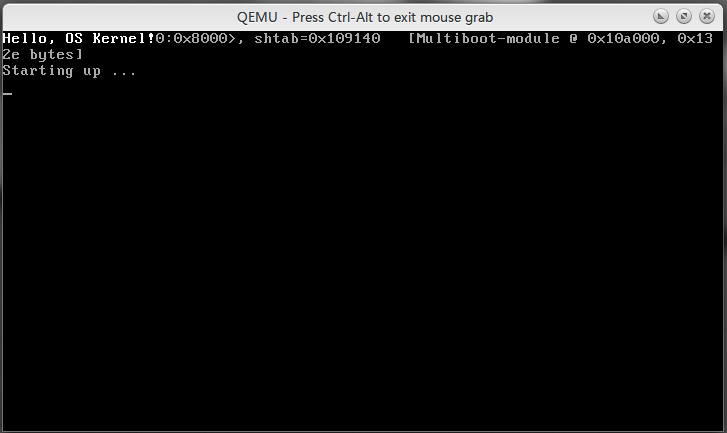
\includegraphics[scale=0.5]{picture/chapt3/hello_os_world.png}
      \caption{虚拟机里运行的 Hello, OS World!}
\end{figure}

\par 至于代码是什么意思大家先不用纠结,下一章将详细探究。

\par 辛苦了这么久,终于看到一点点成功了。有没有一点小兴奋呢?下一章我们将完全的实现对屏幕的字符输出控制,并且有机会\allowbreak
的话我将把这个小内核运行在物理机上,和大家一起体验一下物理机运行的感觉。

\par 真正的好戏从下一章开始,别走开哦。


% 第4章
% -*- coding: UTF-8 -*-
% hurlex-chapt4.tex
% hurlex 开发文档 第4章内容

\section {字符模式下的显卡驱动}

\par 本章将开始描述内核对屏幕输出的控制。

\subsection{1MB以下的地址空间分布}

\par 在第二章我们简单的谈过地址空间的概念,并提到4G的地址空间并非全部指向主存储器,而是有部分的地址分给了其他外设。\allowbreak
特别地,在地址空间的最低1MB处,有很多地址是属于外部设备的,下图描绘了该处地址映射的分布情况:

\begin{figure}[ht]
      \centering
      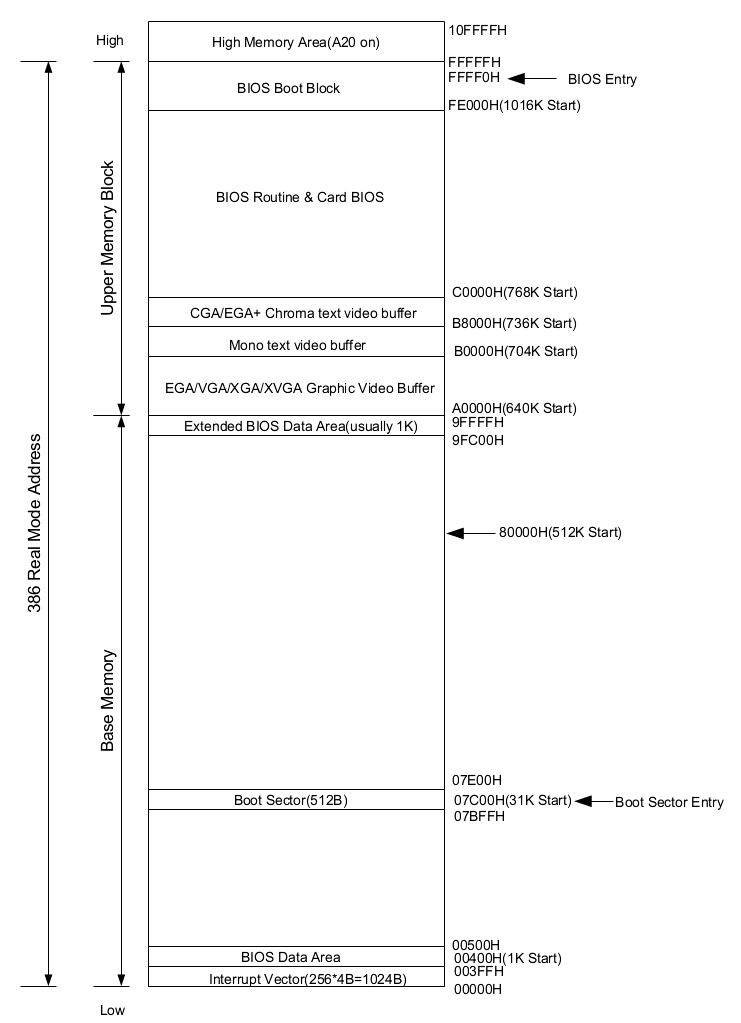
\includegraphics[scale=0.65]{picture/chapt4/BIOS-mem.png}
      \caption{低端地址空间的映射关系}
\end{figure}

\par 在PC上要显示文字,通常需要显示器和显卡这两个硬件设备。一般来说显卡负责提供显示\allowbreak
内容,并控制具体的显示模块和状态。显示器的职责是负责将显卡呈递的内容可视化的显示出来。既然显卡需要控制显示的数据,自然就需要\allowbreak
存储这些待显示的内容,所以显卡就有自己的存储区域。这个存储区域叫做显示存储器(Video RAM,VRAM),简称显存。当然,访问显存\allowbreak
就需要地址。CGA/EGA+ Chroma text video buffer 这个区域映射的就是工作在文本模式的显存。同时显卡还有另外一个工作模式叫做图形\allowbreak
模式,这个模式是目前最最常用的模式。

\subsection{显卡在文本模式下的显示规则}

\par 我们知道,对于一个字符的编码通常有输入码、内码和字模码三种。其中字模码定义了一个字符在屏幕上显示的点阵坐标。通常显卡\allowbreak
内置一套关于基本英文字符的显示是很容易做到的,而内置汉字的显示就较为麻烦。\footnote{曾经有类似于"汉卡"之类的硬件出现,\allowbreak
后来随着计算机处理速度的发展,这些工作一般由软件来负责了。}在这篇文档中我们只使用显卡的文本模式,不会涉及到图形模式的内容。\allowbreak
因为一旦使用了图形模式的内容,我们就需要自行定义字符的字模码了,这很繁琐而且对我们理解操作系统原理的意义不是很大。\allowbreak
所以我们只使用显卡的文本模式进行屏幕显示控制。所有在PC上工作的显卡,在加电初始化之后都会自动初始化到80*25的文本模式。\allowbreak
\footnote{显卡还有其它分辨率的图形工作模式,但本文档不涉及。}\allowbreak
在这个模式下,屏幕被划分为25行,每行可以显示80个字符,所以一屏可以显示2000个字符。上图中的0xB8000~0xBFFFF这个地址段\allowbreak
便是映射到文本模式的显存的。当访问这些地址的时候,实际上读写的是显存区域,而显卡会周期性的读取这里的数据,并且把它们按\allowbreak
顺序显示在屏幕上。

\par 那么,按照什么规则显示呢?这就要谈到内码了。内码定义了字符在内存中存储的形式,而英文编码就是大家所熟知的ASCII\allowbreak
(American Standard Code for Information Interchange,美国信息交换标准代码)码了。对应的关系很简单,从0xB8000这个地址开始,\allowbreak
每2个字节表示屏幕上显示的一个字符。从屏幕的第一行开始对应,一行接着一行的对应下去。而这两个字节的前一个是显示字符的ASCII码,\allowbreak
后一个是控制这个字符颜色和属性的控制信息,这个字节的8个bit位表示不同的含义。每一位的含义如图所示:

\begin{figure}[ht]
      \centering
      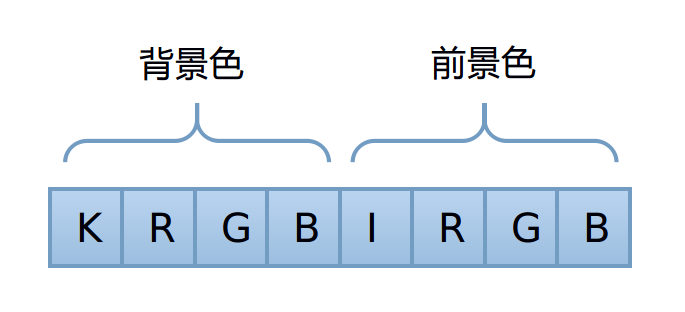
\includegraphics[scale=0.25]{picture/chapt4/char_color.png}
      \caption{字符属性示意图}
\end{figure}

\par 这些位的组合效果如下图所示:

\begin{figure}[ht]
      \centering
      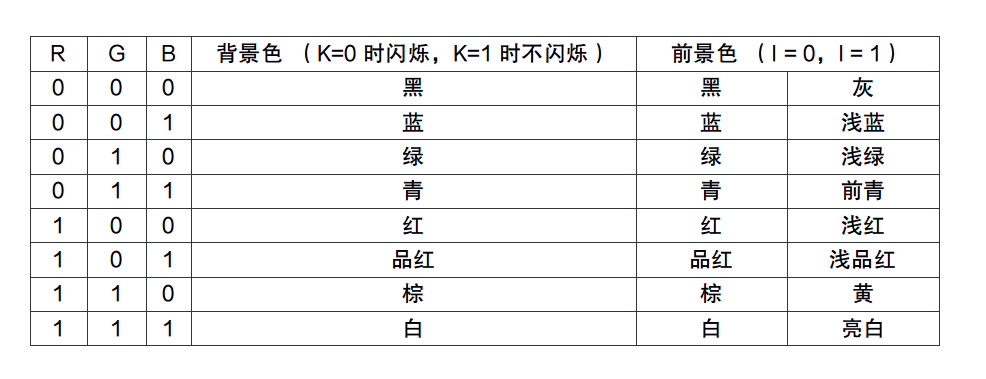
\includegraphics[scale=0.4]{picture/chapt4/text_mode_color.png}
      \caption{显卡文本模式的颜色表}
\end{figure}

\par 这两张图可以帮助我们在显卡的字符模式显示彩色的文本了,懂得这些原理对于探索性质的显示也就足够了。

\par 理解了显卡文本模式的原理之后接下来就是对屏幕显示控制编码了。不过显卡除了显示内容的存储单元之外,还有部分的显示控制\allowbreak
单元需要了解。这些显示控制单元被编制在了独立的I/O空间里,需要用特殊的in/out指令去读写。这里相关的控制寄存器多达300多个,\allowbreak
显然无法一一映射到I/O端口的地址空间。对此工程师们解决方案是,将一个端口作为内部寄存器的索引:0x3D4,再通过0x3D5\allowbreak
端口来设置相应寄存器的值。

\subsection{端口读写函数的实现}

\par 在具体的设置之前,我们首先需要几个端口读写函数的实现。因为C语言并没有直接操作端口的方法,而且频繁的内联汇编麻烦又容易\allowbreak
出错。所以好的做法就是定义几个端口读写函数。代码如下:

\begin{lstlisting}[language = C, caption = libs/common.c]
#include "common.h"

// 端口写一个字节
inline void outb(uint16_t port, uint8_t value)
{
	asm volatile ("outb %1, %0" : : "dN" (port), "a" (value));
}

// 端口读一个字节
inline uint8_t inb(uint16_t port)
{
	uint8_t ret;

	asm volatile("inb %1, %0" : "=a" (ret) : "dN" (port));

	return ret;
}

// 端口读一个字
inline uint16_t inw(uint16_t port)
{
	uint16_t ret;

	asm volatile ("inw %1, %0" : "=a" (ret) : "dN" (port));

	return ret;
}
\end{lstlisting}

\par 对应的头文件如下:
\begin{lstlisting}[language = C, caption = include/common.h]
#ifndef INCLUDE_COMMON_H_
#define INCLUDE_COMMON_H_

#include "types.h"

// 端口写一个字节
void outb(uint16_t port, uint8_t value);

// 端口读一个字节
uint8_t inb(uint16_t port);

// 端口读一个字
uint16_t inw(uint16_t port);

#endif // INCLUDE_COMMON_H_
\end{lstlisting}

\par 细心的读者想必已经发现了函数定义之前的inline关键字了吧?这是GNU对ANSI C的扩展,它和C++语言里的inline的作用是一样的。\allowbreak
函数前面加上inline之后,编译器会尝试\footnote{没错,是尝试。内联对编译来说只是一个建议,编译器有权利根据实际情况自由处理。}\allowbreak
在该函数的调用点进行直接进行代码展开,而不是传统的函数调用。这么做的既有传统函数的好处,即避免了重复性的编码,减少了出错的几率。\allowbreak
又减少了函数的调用,提高了代码的执行效率。另外,你可能见过宏函数这种用法,但是宏函数是没有参数类型的检查的,相比inline还是逊了一筹。

\subsection{颜色的枚举定义和屏幕操作函数的实现}

\par 接下来是颜色定义的枚举和一些屏幕控制函数的声明。代码如下:
\begin{lstlisting}[language = C, caption = include/console.h]
#ifndef INCLUDE_CONSOLE_H_
#define INCLUDE_CONSOLE_H_

#include "types.h"

typedef
enum real_color {
	rc_black = 0,
	rc_blue = 1,
	rc_green = 2,
	rc_cyan = 3,
	rc_red = 4,
	rc_magenta = 5,
	rc_brown = 6,
	rc_light_grey = 7,
	rc_dark_grey = 8,
	rc_light_blue = 9,
	rc_light_green = 10,
	rc_light_cyan = 11,
	rc_light_red = 12,
	rc_light_magenta = 13,
	rc_light_brown  = 14, 	// yellow
	rc_white = 15
} real_color_t;

// 清屏操作
void console_clear();

// 屏幕输出一个字符  带颜色
void console_putc_color(char c, real_color_t back, real_color_t fore);

// 屏幕打印一个以 \0 结尾的字符串  默认黑底白字
void console_write(char *cstr);

// 屏幕打印一个以 \0 结尾的字符串  带颜色
void console_write_color(char *cstr, real_color_t back, real_color_t fore);

// 屏幕输出一个十六进制的整型数
void console_write_hex(uint32_t n, real_color_t back, real_color_t fore);

// 屏幕输出一个十进制的整型数
void console_write_dec(uint32_t n, real_color_t back, real_color_t fore);

#endif  // INCLUDE_CONSOLE_H_
\end{lstlisting}

\par 参照着前面的表格,理解颜色的枚举类型并不困难。接下来是显存起始位置和当前输出的屏幕位置的变量定义。同时,我们将屏幕\allowbreak
抽象为一个80*25的二维数组,每个数组成员都是2个字节,表示屏幕上显示的一个字符。

\begin{lstlisting}[language = C, caption = drivers/console.c]
// VGA 的显示缓冲的起点是 0xB8000
static uint16_t *video_memory = (uint16_t *)0xB8000;

// 屏幕"光标"的坐标
static uint8_t cursor_x = 0;
static uint8_t cursor_y = 0;
\end{lstlisting}

\par 请大家留意这里变量定义时候的 static 限定符,当一个全局变量或者函数只在本模块文件内被使用时,最好限定其作用域。每个模块\allowbreak
应当尽可能的向外部暴露较少的接口。

\subsubsection{屏幕输入光标的移动}

\par 在本模块内,cursor\_x 和 cursor\_y 这两个变量指明了逻辑上的当前输出位置,但是并没有实际上移动硬件的显示"光标",\allowbreak
下面的函数实现了根据这两个变量的值移动光标的功能。

\begin{lstlisting}[language = C, caption = drivers/console.c]
static void move_cursor()
{
	// 屏幕是 80 字节宽
	uint16_t cursorLocation = cursor_y * 80 + cursor_x;
	
	// 在这里用到的两个内部寄存器的编号为14与15,分别表示光标位置
	// 的高8位与低8位。

	outb(0x3D4, 14); 			// 告诉 VGA 我们要设置光标的高字节
	outb(0x3D5, cursorLocation >> 8); 	// 发送高 8 位
	outb(0x3D4, 15); 			// 告诉 VGA 我们要设置光标的低字节
	outb(0x3D5, cursorLocation);      	// 发送低 8 位
}
\end{lstlisting}

\par 这里的端口和设置值都是固定的,也没有什么道理可讲。虽然显卡的各项技术发展的很快,但是这个原始的VGA标准被所有显卡完整\allowbreak
的保存了下来。

\subsubsection{清屏操作}

\par 然后是清屏操作,其实这里的"清屏"很简单,其实就是用白底黑字的"空格符"覆盖整个屏幕的显示区域罢了。这么做自然就实现了\allowbreak
我们想要的"清屏"操作了。代码很简单:

\begin{lstlisting}[language = C, caption = drivers/console.c]
void console_clear()
{
	uint8_t attribute_byte = (0 << 4) | (15 & 0x0F);
	uint16_t blank = 0x20 | (attribute_byte << 8);

	int i;
	for (i = 0; i < 80 * 25; i++) {
	      video_memory[i] = blank;
	}

	cursor_x = 0;
	cursor_y = 0;
	move_cursor();
}
\end{lstlisting}

\subsubsection{屏幕滚动显示}

\par 那么屏幕滚动呢?用C语言来描述实际上就是将后24行的数据全部向上挪动一行,最后一行清空罢了,就是这么简单。

\begin{lstlisting}[language = C, caption = drivers/console.c]
static void scroll()
{
	// attribute_byte 被构造出一个黑底白字的描述格式
	uint8_t attribute_byte = (0 << 4) | (15 & 0x0F);
	uint16_t blank = 0x20 | (attribute_byte << 8);  // space 是 0x20

	// cursor_y 到 25 的时候,就该换行了
	if (cursor_y >= 25) {
		// 将所有行的显示数据复制到上一行,第一行永远消失了...
		int i;
		
		for (i = 0 * 80; i < 24 * 80; i++) {
		      video_memory[i] = video_memory[i+80];
		}

		// 最后的一行数据现在填充空格,不显示任何字符
		for (i = 24 * 80; i < 25 * 80; i++) {
		      video_memory[i] = blank;
		}
		
		// 向上移动了一行,所以 cursor_y 现在是 24
		cursor_y = 24;
	}
}
\end{lstlisting}

\subsubsection{显示字符串}

\par 那么屏幕显示字符串呢?我们可以先实现屏幕显示一个字符的函数,那么屏幕显示一个字符串不就可以了么。这几个函数的实现如下:

\begin{lstlisting}[language = C, caption = drivers/console.c]
void console_putc_color(char c, real_color_t back, real_color_t fore)
{
	uint8_t back_color = (uint8_t)back;
	uint8_t fore_color = (uint8_t)fore;

	uint8_t attribute_byte = (back_color << 4) | (fore_color & 0x0F);
	uint16_t attribute = attribute_byte << 8;

	// 0x08 是退格键的 ASCII 码
	// 0x09 是tab 键的 ASCII 码
	if (c == 0x08 && cursor_x) {
	      cursor_x--;
	} else if (c == 0x09) {
	      cursor_x = (cursor_x+8) & ~(8-1);
	} else if (c == '\r') {
	      cursor_x = 0;
	} else if (c == '\n') {
		cursor_x = 0;
		cursor_y++;
	} else if (c >= ' ') {
		video_memory[cursor_y*80 + cursor_x] = c | attribute;
		cursor_x++;
	}

	// 每 80 个字符一行,满80就必须换行了
	if (cursor_x >= 80) {
		cursor_x = 0;
		cursor_y ++;
	}

	// 如果需要的话滚动屏幕显示
	scroll();

	// 移动硬件的输入光标
	move_cursor();
}

void console_write(char *cstr)
{
	while (*cstr) {
	      console_putc_color(*cstr++, rc_black, rc_white);
	}
}

void console_write_color(char *cstr, real_color_t back, real_color_t fore)
{
	while (*cstr) {
	      console_putc_color(*cstr++, back, fore);
	}
}
\end{lstlisting}

\par 代码里唯一需要注意的便是输出后要检查当前的位置和判断一些特殊的符号表示的操作,例如换行之类的实现。同时一定要注意修改存储\allowbreak
当前位置的两个变量和移动屏幕上的光标,而且屏幕输出满了以后要上滚。我们暂时不考虑诸如屏幕翻页之类的功能。至于屏幕输出十六进制\allowbreak
数字和十进制数字的函数请大家自己实现,相信这并不困难。

\subsection{测试屏幕操作函数}

\par 屏幕的操作到这里就告一段落了,我们修改下初始化函数,感受一下今天的成果吧。

\begin{lstlisting}[language = C, caption = init/entry.c]
#include "console.h"

int kern_entry(multiboot_t *mboot_ptr)
{
	console_clear();

	console_write_color("Hello, OS kernel!\n", rc_black, rc_green);

	return 0;
}
\end{lstlisting}

\par 编译运行,干净的屏幕上出现了我们绿色的文字,还有下一行闪烁着的输入光标。

\begin{figure}[ht]
      \centering
      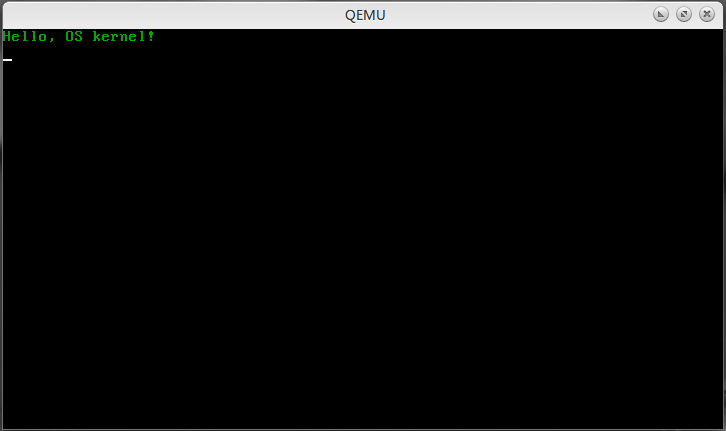
\includegraphics[scale=0.5]{picture/chapt4/hello_os_world_green.png}
      \caption{屏幕输出控制的展示}
\end{figure}

\par 本章的内容到这里就结束了,下一章我们缓缓脚步,来完成一些更重要的模块。


% 第5章
% -*- coding: UTF-8 -*-
% hurlex-chapt5.tex
% hurlex 开发文档 第5章内容

\section {相关库函数和调试打印函数}


\begin{lstlisting}[language = C, label = include/multiboot.h, caption = include/multiboot.h]
#ifndef INCLUDE_MULTIBOOT_H_
#define INCLUDE_MULTIBOOT_H_

#include "types.h"

typedef
struct multiboot_t {
	uint32_t flags;		// Multiboot 的版本信息
	uint32_t mem_lower;
	uint32_t mem_upper;
	uint32_t boot_device;
	uint32_t cmdline;	// 内核命令行
	uint32_t mods_count;	// boot 模块列表
	uint32_t mods_addr;
	uint32_t num;
	uint32_t size;
	uint32_t addr;
	uint32_t shndx;

	uint32_t mmap_length;		
	uint32_t mmap_addr;
	
	uint32_t drives_length; // 指出第一个驱动器结构的物理地址	
	uint32_t drives_addr; 	// 指出第一个驱动器这个结构的大小
	uint32_t config_table; 	// ROM 配置表
	uint32_t boot_loader_name; 	// boot loader 的名字
	uint32_t apm_table; 	    	// APM 表
	uint32_t vbe_control_info;
	uint32_t vbe_mode_info;
	uint32_t vbe_mode;
	uint32_t vbe_interface_seg;
	uint32_t vbe_interface_off;
	uint32_t vbe_interface_len;
} __attribute__((packed)) multiboot_t;

typedef
struct mmap_entry_t {
	uint32_t size; 	// 留意 size 是不含 size 自身变量的大小
	uint32_t base_addr_low;
	uint32_t base_addr_high;
	uint32_t length_low;
	uint32_t length_high;
	uint32_t type;
} __attribute__((packed)) mmap_entry_t;

// 声明全局的 multiboot_t * 指针
extern multiboot_t *glb_mboot_ptr;

#endif 	// INCLUDE_MULTIBOO
\end{lstlisting}

% 第6章
% -*- coding: UTF-8 -*-
% hurlex-chapt6.tex
% hurlex 开发文档 第6章内容

\section {添加全局段描述符表}

\subsection{保护模式的引入}

\par 从本章开始,我们就要开始涉及到x86保护模式编程的一些细节问题了。

\par 我们从80386处理器入手。首先,到了80386时代,CPU有了四种运行模式,即实模式、保护模式、虚拟8086模式和SMM模式。

\par 模式指的是8086CPU的运行模式,不过这是后来提出的概念,在8086时代只有当时的运行模式,自然也就没有"实模式"这么个提法。\allowbreak
如果世界上只有一种性别的人,也就没有男人,女人这种名称了。8086的汇编中,我们对于实模式的各种机制应该算是比较了解了,其\allowbreak
大致包括实模式1MB的线性地址空间、内存寻址方法、寄存器、端口读写以及中断处理方法等内容。

\par 不过到了80386时代,引进了一种沿用至今的CPU运行机制——保护模式(Protected Mode)。保护模式有一些新的特色,用来增强多工\allowbreak
和系统稳定度,比如内存保护,分页系统,以及硬件支持的虚拟内存等。大部分现今基于x86架构的操作系统都在保护模式下运行,\allowbreak
包括Linux、FreeBSD、以及微软Windows 2.0和之后版本(都指32位操作系统) 。

\par 虚拟8086模式用于在保护模式下运行原来实模式下的16位程序,我们不关心。SMM模式是不对程序员开放的,所以我们也不关心。

\par 我们先来研究保护模式,在保护模式里80386首先扩展了8086的处理器\footnote{其实中间有个80286,不过这是个过渡产品。},\allowbreak
原先的AX,BX,CX,DX,SI,DI,SP,BP从16位扩展(Extend)到了32位,并改名EAX,EBX,ECX,EDX,ESI,EDI,ESP,EBP,E\allowbreak
就是Extend的意思。当然,保留了原先的16位寄存器的使用习惯,就像在8086下能用AH和AL访问AX的高低部分一样,不过EAX的低\allowbreak
位部分能使用AX直接访问,高位却没有直接的方法,只能通过数据右移16位之后再访问。另外,CS,DS,ES,SS这几个16位段寄存器\allowbreak
保留,再增加FS,GS两个段寄存器。另外还有其它很多新增加的寄存器。本着实用原则,到时候用到了我们再说。

\subsection{保护模式下的内存分段}

\par 我们知道,对CPU来讲,系统中的所有储存器中的储存单元都处于一个统一的逻辑储存器中,它的容量受CPU寻址能力的限制。\allowbreak
这个逻辑储存器就是我们所说的线性地址空间。8086有20位地址线,拥有1MB的线性地址空间。而80386有32位地址线,拥有4GB的\allowbreak
线性地址空间。但是80386依旧保留了8086采用的地址分段的方式,只是增加了一个折中的方案,即只分一个段,段基址0×00000000,\allowbreak
段长0xFFFFFFFF(4GB),这样的话整个线性空间可以看作就一个段,这就是所谓的平坦模型(Flat Mode)。

\par  我们先来看保护模式下的内存是如何分段管理的。为了便于理解,我们从一个设计者的角度来研究这个问题,顺便试图按我的理\allowbreak
解对一些机制的设计原因做一些阐释。

\par 首先是对内存分段中每一个段的描述,内模式对于内存段并没有访问控制,任意的程序可以修改任意地址的变量,而保护模式需要\allowbreak
对内存段的性质和允许的操作给出定义,以实现对特定内存段的访问检测和数据保护。考虑到各种属性和需要设置的操作,32位保护模式\allowbreak
下对一个内存段的描述需要8个字节,其称之为段描述符(Segment Descriptor)。段描述符分为数据段描述符、指令段描述符\allowbreak
和系统段描述符三种。

\par 我们现在看一张段描述符的8个字节的分解图吧,至于每一个细节的含义请大家自行查阅Intel文档。\allowbreak
\footnote{本章很多图片直接引用自《Intel® 64 and IA-32 Architectures Software Developer’s Manual Vol-ume3 :
System Programming Guide》,下文不再声明。}

\begin{figure}[ht]
      \centering
      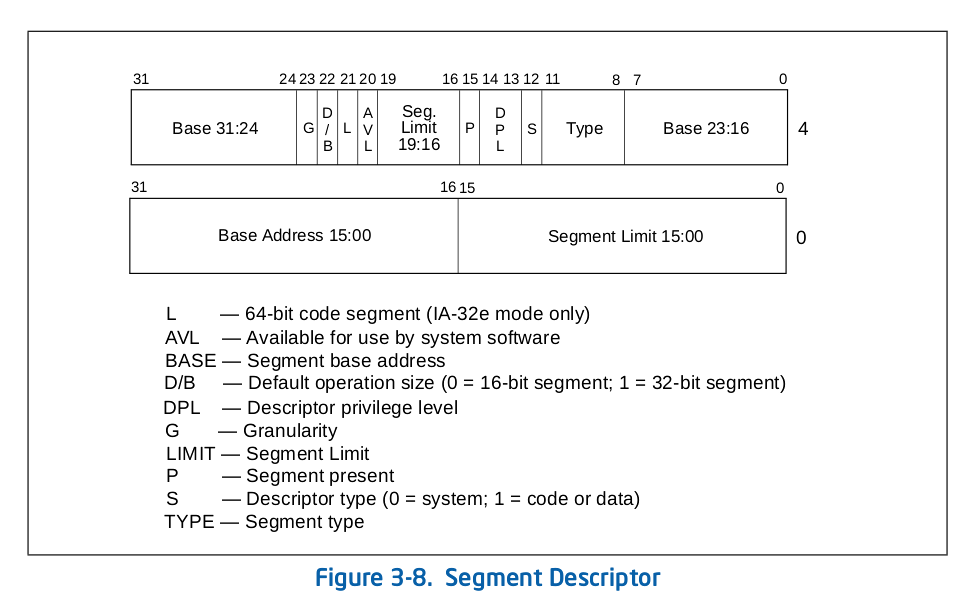
\includegraphics[scale=0.45]{picture/chapt6/segment_descriptor.png}
      \caption{段描述符的结构}
\end{figure}

 \par 显然,寄存器不足以存放N多个内存段的描述符集合,所以这些描述符的集合(称之为描述符表)被放置在内存里了。\allowbreak
 在很多描述符表中,最重要的就是所谓的全局描述符表(Global Descriptor Table,GDT),它为整个软硬件系统服务。

 \par 一个问题解决了,但是又引出了的其他问题。问题一:这些描述符表放置在内存哪里?答案是没有固定的位置,可以任由\allowbreak
 程序员安排在任意合适的位置。问题一带出了问题二:既然没有指定固定位置,CPU如何知道全局描述符表在哪?答案是Intel干脆设置了\allowbreak
 一个48位的专用的全局描述符表寄存器(GDTR)来保存全局描述符表的信息。那这48位怎么分配呢?如图所示,0-15位表示GDT\allowbreak
 的边界位置(数值为表的长度-1,因为从0计算),16-47位这32位存放的就是GDT的基地址(恰似数组的首地址)。

\begin{figure}[ht]
      \centering
      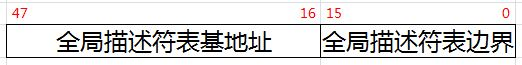
\includegraphics[scale=0.5]{picture/chapt6/gdtr.png}
      \caption{GDTR的结构}
\end{figure}

\par 既然用16位来表示表的长度,那么2的16次方就是65536字节,除以每一个描述符的8字节,那么最多能创建8192个描述符。

\par 貌似说了这么多,我们一直还没提CPU的默认工作方式。80386CPU加电的时候自动进入实模式\footnote{实际上此时CPU还不是\allowbreak
彻底的实模式,之后第二条指令才进入彻底的实模式。对这个问题的讨论超出本文档的范围,所以不再讨论。}既然CPU加电后就一直\allowbreak
工作在实模式下了。那怎么进入保护模式呢?说来也简单,80386CPU内部有5个32位的控制寄存器(Control Register,CR),\allowbreak
分别是CR0到CR3,以及CR8。用来表示CPU的一些状态,其中的CR0寄存器的PE位(Protection Enable,保护模式允许位),0号位,\allowbreak
就表示了CPU的运行状态,0为实模式,1为保护模式。通过修改这个位就可以立即改变CPU的工作模式。

\begin{figure}[ht]
      \centering
      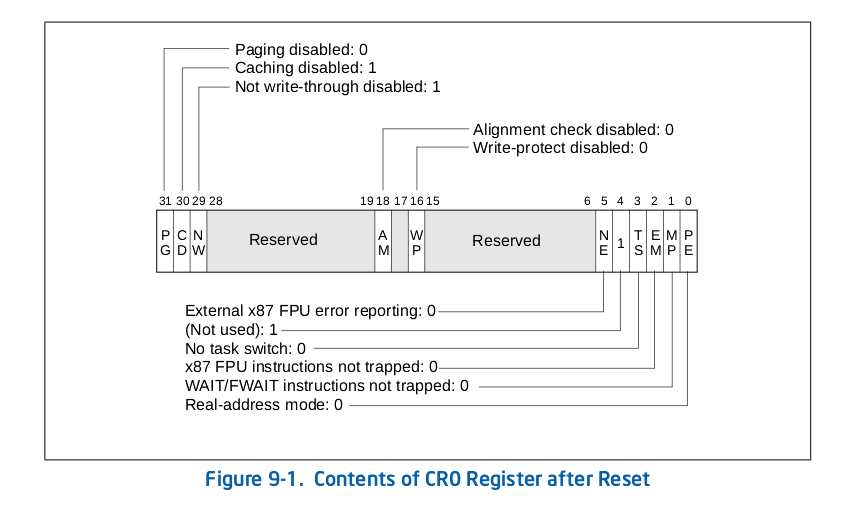
\includegraphics[scale=0.5]{picture/chapt6/cr0.png}
      \caption{CR0寄存器的结构}
\end{figure}

\par 不过需要注意的是,一旦CR0寄存器的PE位被修改,CPU就立即按照保护模式去寻址了,所以这就要求我们必须在进入保护模式\allowbreak
之前就在内存里放置好GDT,然后设置好GDTR寄存器。我们知道实模式下只有1MB的寻址空间,所以GDT就等于被限制在了这里。即便\allowbreak
是再不乐意我们也没有办法,只得委屈就全的先安排在这里。不过进入保护模式之后我们就可以在4G的空间里设置并修改原来的GDTR了。

\par OK,现在有了描述符的数组了,也有了“数组指针”(GDTR)了,怎么表示我们要访问哪个段呢?还记得8086时代的段寄存器吧?\allowbreak
不过此时它们改名字了,叫段选择器(段选择子)。此时的CS等寄存器不再保存段基址了,而是保存其指向段的索引信息,CPU会根据\allowbreak
这些信息在内存中获取到段信息。

\par 地址合成的过程如下图所示:

\begin{figure}[ht]
      \centering
      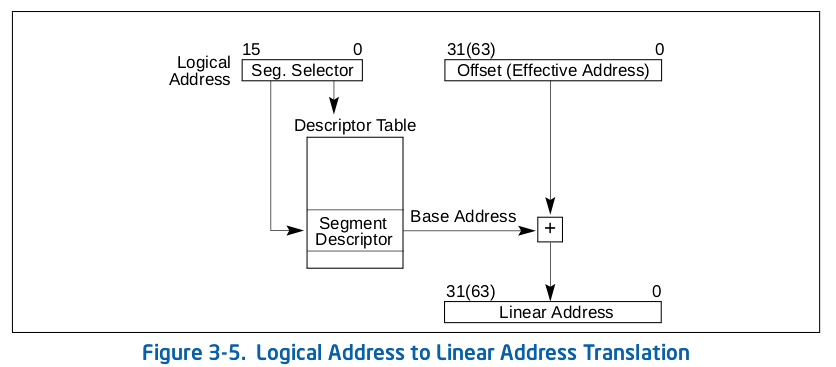
\includegraphics[scale=0.5]{picture/chapt6/protected_segment_addr.png}
      \caption{段机制的地址合成过程}
\end{figure}

\par 以上就是对x86保护模式的阐述了,细节问题希望大家能结合之后的代码自行参考Intel文档学习。

\subsection{具体采用的分段策略}

\par 下面开始针对我们的内核给出具体的设计方案了。我们之前简单的阐述了分段,事实上现代操作系统几乎不再使用分段而是绕过\allowbreak
分段技术直接使用了分页。其实分段和分页没什么必然联系。只不过Intel从8086开始,其制造的CPU就以段地址+偏移地址的方式来访问内存。\allowbreak
后来要兼容以前的CPU,Intel不得不一直保留着这个传统。分段可以说是Intel的CPU一直保持着的一种机制,而分页只是保护模式下\allowbreak
的一种内存管理策略。不过想开启分页机制,CPU就必须工作在保护模式,而工作在保护模式时候可以不开启分页。所以事实上分段是\allowbreak
必须的,而分页是可选的。

\par 那我们如何"绕过"这个分段机制呢?不知道大家是否还记得之前我们所说的平坦模式(Flat Mode)?这就是我们"绕过"的\allowbreak
方法。当整个虚拟地址空间是一个起始地址为0,限长为4G的"段"时,我们给出的偏移地址就在数值上等于是段机制处理之后的地址了。
不过我们不是简单的对所有的段使用同样的描述符,而是给代码段和数据段分配不同的描述符。下面的示意图描述了这个抽象:

\begin{figure}[ht]
      \centering
      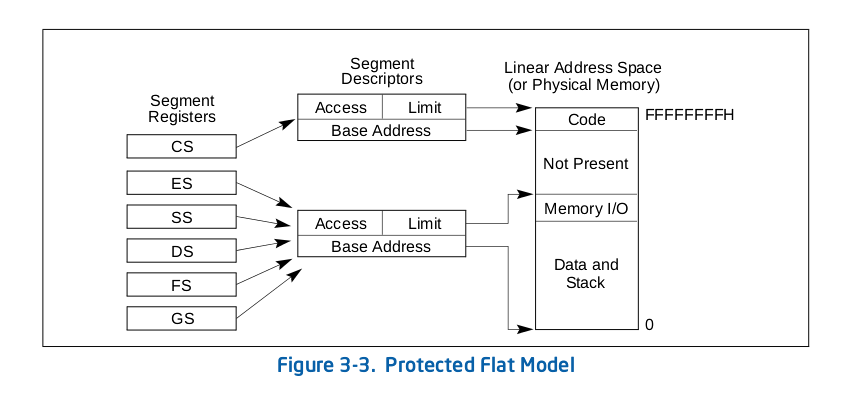
\includegraphics[scale=0.5]{picture/chapt6/protected_flat_mode.png}
      \caption{带有保护的平坦模式}
\end{figure}

\par 在第二章中我们谈到了GRUB在载入内核时候的一些状态,其中就有以下两条:

\begin{mdframed}
	\begin{enumerate}
		\item CS 指向基地址为 0x00000000,限长为4G – 1的代码段描述符。
		\item DS,SS,ES,FS 和 GS 指向基地址为0x00000000,限长为4G–1的数据段描述符。
	\end{enumerate}
\end{mdframed}

\par 大家现在应该了理解这两项了吧?既然GRUB已经替我们做过了,那我们还有必要再来一次吗?当然有必要了,一来是学习的必要,\allowbreak
二来在后期实现TSS任务切换的时候还要用到全局描述符表。

\par 下面我们给出具体的实现代码,首先是头文件和一些定义:

\begin{lstlisting}[language = C, caption = include/gdt.h]
#ifndef INCLUDE_GDT_H_
#define INCLUDE_GDT_H_

#include "types.h"

// 全局描述符类型
typedef
struct gdt_entry_t {
	uint16_t limit_low;     // 段界限   15 ~ 0
	uint16_t base_low;      // 段基地址 15 ~ 0
	uint8_t  base_middle;   // 段基地址 23 ~ 16
	uint8_t  access;        // 段存在位、描述符特权级、描述符类型、描述符子类别
	uint8_t  granularity; 	// 其他标志、段界限 19 ~ 16
	uint8_t  base_high;     // 段基地址 31 ~ 24
} __attribute__((packed)) gdt_entry_t;

// GDTR
typedef
struct gdt_ptr_t {
	uint16_t limit; 	// 全局描述符表限长
	uint32_t base; 		// 全局描述符表 32 位基地址
} __attribute__((packed)) gdt_ptr_t;

// 初始化全局描述符表
void init_gdt();

// GDT 加载到 GDTR 的函数[汇编实现]
extern void gdt_flush(uint32_t);

#endif 	// INCLUDE_GDT_H_
\end{lstlisting}

\par 结合上面关于全局段描述符表的格式说明,这两个结构体的定义应该很容易看懂。具体的函数实现如下:

\begin{lstlisting}[language = C, caption = gdt/gdt.c]
#include "gdt.h"
#include "string.h"

// 全局描述符表长度
#define GDT_LENGTH 5

// 全局描述符表定义
gdt_entry_t gdt_entries[GDT_LENGTH];

// GDTR
gdt_ptr_t gdt_ptr;

static void gdt_set_gate(int32_t num, uint32_t base,
			uint32_t limit, uint8_t access, uint8_t gran);

// 声明内核栈地址
extern uint32_t stack;

// 初始化全局描述符表
void init_gdt()
{
	// 全局描述符表界限 e.g. 从 0 开始,所以总长要 - 1
	gdt_ptr.limit = sizeof(gdt_entry_t) * GDT_LENGTH - 1;
	gdt_ptr.base = (uint32_t)&gdt_entries;

	// 采用 Intel 平坦模型
	gdt_set_gate(0, 0, 0, 0, 0);   // 按照 Intel 文档要求,第一个描述符必须全 0
	gdt_set_gate(1, 0, 0xFFFFFFFF, 0x9A, 0xCF); 	// 指令段
	gdt_set_gate(2, 0, 0xFFFFFFFF, 0x92, 0xCF); 	// 数据段
	gdt_set_gate(3, 0, 0xFFFFFFFF, 0xFA, 0xCF); 	// 用户模式代码段
	gdt_set_gate(4, 0, 0xFFFFFFFF, 0xF2, 0xCF); 	// 用户模式数据段

	// 加载全局描述符表地址到 GPTR 寄存器
	gdt_flush((uint32_t)&gdt_ptr);
}

// 全局描述符表构造函数,根据下标构造
// 参数分别是 数组下标、基地址、限长、访问标志,其它访问标志
static void gdt_set_gate(int32_t num, uint32_t base, uint32_t limit, uint8_t access, uint8_t gran)
{
	gdt_entries[num].base_low     = (base & 0xFFFF);
	gdt_entries[num].base_middle  = (base >> 16) & 0xFF;
	gdt_entries[num].base_high    = (base >> 24) & 0xFF;

	gdt_entries[num].limit_low    = (limit & 0xFFFF);
	gdt_entries[num].granularity  = (limit >> 16) & 0x0F;

	gdt_entries[num].granularity |= gran & 0xF0;
	gdt_entries[num].access       = access;
}

\end{lstlisting}

\par 这里唯一麻烦的就是需要对照着Intel文档的说明,去为每一个段描述符计算权限位的数值了。\allowbreak
至于加载全局描述符表的操作,为了方便期间我们直接用汇编语言实现了,代码如下:\allowbreak
\footnote{这里需要强调的是这里的代码文件命名为gdt\_s.s,因为同一个目录下的.s和.c文件都会被编译为同名的.o文件,所以同名的话\allowbreak
会被相互覆盖掉。}

\begin{lstlisting}[language = {[x86masm]Assembler}, caption = gdt/gdt\_s.s]
[GLOBAL gdt_flush]

gdt_flush:
	mov eax, [esp+4]  ; 参数存入 eax 寄存器
	lgdt [eax]        ; 加载到 GDTR [修改原先GRUB设置]

	mov ax, 0x10      ; 加载我们的数据段描述符
	mov ds, ax        ; 更新所有可以更新的段寄存器
	mov es, ax
	mov fs, ax
	mov gs, ax
	mov ss, ax
	jmp 0x08:.flush   ; 远跳转, 0x08 是我们的代码段描述符
			  ; 远跳目的是清空流水线并串行化处理器
.flush:
	ret
\end{lstlisting}

\par 我想这个汇编函数中唯一需要解释的就是jmp跳转那一句了,首先0×08是我们跳转目标段的段选择子(这个不陌生吧?),\allowbreak
其对应段描述符第2项。后面的跳转目标标号可能会让你诧异,因为它就是下一行代码。这是为何?当然有深意了,第一,Intel不\allowbreak
允许直接修改段寄存器cs的值,我们只好这样通过这种方式更新cs段寄存器;第二,x86以后CPU所增加的指令流水线和高速缓存可能\allowbreak
会在新的全局描述符表加载之后依旧保持之前的缓存,那么修改GDTR之后最安全的做法就是立即清空流水线和更新高速缓存。说的这么\allowbreak
牛逼的样子,其实只要一句jmp跳转就能强迫CPU自动更新了,很简单吧?

\par 到这里段描述符表的创建就告一段落了,其实我们完全可以直接计算出这些段具体的表示数值然后硬编码进去,但是出于学习的\allowbreak
目的,我们还是写了这些函数进行处理。当然了,我们没有谈及一些具体的描述符细节问题,因为Intel文档的描述都很详细。

\par 创建好所有的文件以后,再次修改入口函数如下:

\begin{lstlisting}[language = C, caption = init/entry.c]
#include "gdt.h"
#include "console.h"
#include "debug.h"

int kern_entry()
{
	init_debug();
	init_gdt();

	console_clear();
	printk_color(rc_black, rc_green, "Hello, OS kernel!\n");

	return 0;
}
\end{lstlisting}

\par 编译运行后如果输出了正常的信息,就说明我们成功了。于是,本章结束。

% 第7章
% -*- coding: UTF-8 -*-
% hurlex-chapt7.tex
% hurlex 开发文档 第7章内容

\section {添加中断描述符表}

\subsection{中断的引入}

\par 中断是用以提高计算机工作效率、增强计算机功能的一项重要技术。其实简单说中断就是一种通知机制罢了。我们知道操作系统的一个\allowbreak
核心任务就是和连接在主板上的所有的硬件设备进行通信,但是CPU和这些外设的速率根本就不在一个数量级上,倘若CPU向某一个设备发出一\allowbreak
个请求并且一直等待反馈结果的话,这样带来的性能损失是不可接受的。而且CPU在运行期间需要得知外设所发生的事件,轮询显然是不可取\allowbreak
的,那么就迫切需要一种机制来帮助我们解决这个问题。

\par 肩负着这一伟大使命,中断应运而生。当某个中断发生时,典型的处理方式就是CPU会打断当前的任务,保留当前的执行现场后再\allowbreak
转移到该中断事先安排好的中断处理函数\footnote{或者叫中断服务例程。}去执行。在中断处理函数执行结束之后再恢复中断之前的执\allowbreak
行现场,去执行之前的任务。

\par 从物理学的角度看,中断其实就是一种电信号,一般由硬件设备生成并送入中断控制器统一协调\footnote{当然需要一个"协调机构"了,\allowbreak\
试想所有设备不区分轻重缓急的和CPU发送中断信号的恐怖场景…}。中断控制器就是个简单的电子芯片,其作用就是将汇集的多路中断管线,采用\allowbreak
复用技术只通过一条中断线和CPU相连接。既然中断控制器这里只有一条线和CPU相链接,那么为了区分各个设备,中断自然就有编号了。

\par 补充一下,其实CPU的中断管脚并非只有一根,其实是有NMI和INTR两个管脚,因为从严重性上来看,中断是分为两类的,首先NMI管脚触发的\allowbreak
中断是需要无条件立即处理的,这种类型的中断是不会被阻塞和屏蔽的,所以叫做非屏蔽中断(Non Maskable Interrupt, NMI)。\allowbreak
事实上一旦产生了NMI中断,就意味着CPU遇到了不可挽回的错误,一般不会进行处理,只是给出一个错误信息。而我们之前所说的中断\allowbreak
控制器连接的管脚叫做INTR,这类中断有两个特点,分别是数量多和可屏蔽。而我们主要关注的正是INTR中断。

\par 举一个通俗的例子,假设你就是CPU,你正在看书(执行任务),突然间你的鼻涕流下来了(一个NMI中断),这个自然是不可以屏蔽的,\allowbreak
不然会流到嘴里的…(好恶心),你现在把书反着扣在桌子上避免找不到页码(保留当前执行现场),取出纸巾…(此处省略几十个字),OK,\allowbreak
你处理完后把书拿起来继续看(恢复之前的执行现场)。这就是一个中断的处理过程,其实很简单是不是?这是不可屏蔽中断,那么可屏蔽\allowbreak
的呢?还是刚刚那个场景,你在看书,手机响了(一个INTR中断),但是你在学习期间不想被打扰,就无视它了…这就是可屏蔽中断了。

\par 通俗的例子举完了,我们还是专业一点好了。在x86PC中,我们熟知的中断控制芯片就是8259A PIC了,它就是我们说的中断控制器了。Intel的\allowbreak
处理器允许256个中断,中断号范围是0~255。8259A PIC芯片负责15个,但是并不固定中断号,允许通过IO端口设置以避免冲突。它的全称\allowbreak
是可编程中断控制器(Programmable Interrupt Controller,PIC)。关于8259A PIC的资料网上铺天盖地的,至于8259A PIC的结构,\allowbreak
如何屏蔽中断什么的我就不多说了,请大家自行去了解。

\par 其实从上面的描述中我们基本上能理解中断的概念了。再简单说就是硬件发生了某个事件后告诉中断控制器,中断控制器汇报给CPU,\allowbreak
CPU从中断控制器处得知了中断号,根据这个中断号找到对应的中断处理程序并转移过去执行,完成后重新回到之前的执行流程去。

\par 我们之前一直说的都是硬件中断,其实除了硬件中断之外还有软件中断,也就是软件系统也可以利用中断机制来完成一些任务,\allowbreak
比如有些OS的系统调用的实现就采用了中断的方式。

\subsection{中断的实现}

\par 我们的重点是保护模式下的中断处理。中断处理程序是运行在ring0层的,这就意味着中断处理程序拥有着系统的全部权限,仿照内存段\allowbreak
描述符表的思路,Intel设置了一个叫做中断描述符表(IDT, Interrupt Descriptor Table)的东西,和段描述符表一样放置在主存中,\allowbreak
类似地,也有一个中断描述符表寄存器(IDTR)记录这个表的起始地址。那么下文的重点就是这个中断描述符的结构和设置方法了,其实\allowbreak
这里很类似GDT的那一套过程,我们先给出中断描述符表的结构:\allowbreak
\footnote{照例引用Intel文档中的插图,这是一篇开源的文档,应该没有版权纠纷吧...}

\begin{figure}[ht]
      \centering
      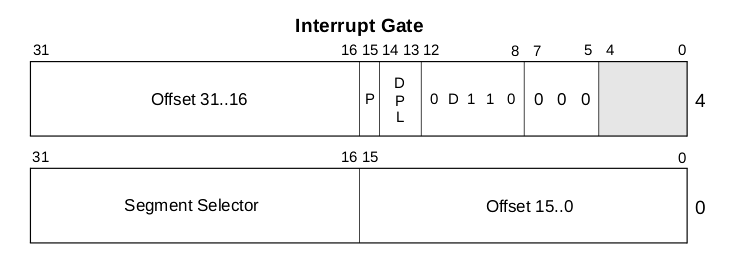
\includegraphics[scale=0.5]{picture/chapt7/interrupt_gate.png}
      \caption{中断描述符的格式}
\end{figure}

\par 根据这个描述信息,我们给出相关的C语言结构体定义:

\begin{lstlisting}[language = C, caption = include/idt.h]
#ifndef INCLUDE_IDT_H_
#define INCLUDE_IDT_H_

#include "types.h"

// 初始化中断描述符表
void init_idt();

// 中断描述符
typedef
struct idt_entry_t {
	uint16_t base_lo;        // 中断处理函数地址 15 ~ 0 位
	uint16_t sel;            // 目标代码段描述符选择子
	uint8_t  always0;        // 置 0 段
	uint8_t  flags;          // 一些标志,文档有解释
	uint16_t base_hi;        // 中断处理函数地址 31 ~ 16 位
}__attribute__((packed)) idt_entry_t;

// IDTR
typedef
struct idt_ptr_t {
	uint16_t limit; 	// 限长
	uint32_t base; 		// 基址
} __attribute__((packed)) idt_ptr_t;

#endif 	// INCLUDE_IDT_H_
\end{lstlisting}

\par 之前我们建立了中断的概念并且介绍了描述符表的结构,接下来我们细化CPU处理中断的\allowbreak
过程,首先是起始过程,也就是从CPU发现中断事件后,打断当前程序或任务的执行,根据某种机制跳转到中断处理函数去执行的过程:
\begin{enumerate}
	\item CPU在执行完当前程序的每一条指令后,都会去确认在执行刚才的指令过程中是否发送中断请求过来,如果有那么CPU\allowbreak
		就会在相应的时钟脉冲到来时从总线上读取中断请求对应的中断向量。然后根据得到的中断向量为索引到IDT中找到该向量\allowbreak
		对应的中断描述符,中断描述符里保存着中断处理函数的段选择子;
	\item CPU使用IDT查到的中断处理函数段选择子从GDT中取得相应的段描述符,段描述符里保存了中断处理函数的段基址和属性信息。\allowbreak
		此时CPU要进行一个很关键的特权检验的过程,这个涉及到CPL、RPL和DPL的数值检验以及判断是否发生用户态到内核态的切换。\allowbreak
		如果发生了切换,还要涉及到TSS段和用户栈和内核栈的切换;\footnote{这些东西我们之前都没有说过,所以大家看不懂的话\allowbreak
		就先跳过去,等到后面讲到保护环的时候我们再细说。}
	\item 确认无误后CPU开始保存当前被打断的程序的现场(即一些寄存器的值),以便于将来恢复被打断的程序继续执行。这需要利用内核栈来保存\allowbreak
		相关现场信息,即依次压入当前被打断程序使用的eflags、cs、eip、以及错误代码号(如果当前中断有错误代码);
	\item 最后CPU会从中断描述符中取出中断处理函数的起始地址并跳转过去执行。
\end{enumerate}

\par 以上是起始过程,中断处理函数执行完成之后需要通过iret或iretd指令恢复被打断的程序的执行。这时候比较简单,首先CPU会从内核栈\allowbreak
里弹出先前保存的被打断的程序的现场信息,即之前的eflags,cs,eip重新开始被打断前的任务。\allowbreak
\footnote{如果之前存在特权级转换(从内核态转换到用户态),则还需要从内核栈中弹出用户态栈的ss和esp,这样也意味着\allowbreak
栈也被切换回原先使用的用户态的栈了。}
\par 需要注意的是:如果此次处理的是带有错误码的中断,CPU 在恢复先前程序的现场时,并不会弹出错误代码。\allowbreak
这一步需要通过软件完成,即要求相关的中断处理函数在使用iret指令返回之前添加出栈代码主动弹出错误代码。

\par 下图描述了CPU自动保护和恢复的寄存器的栈结构:
\begin{figure}[ht]
      \centering
      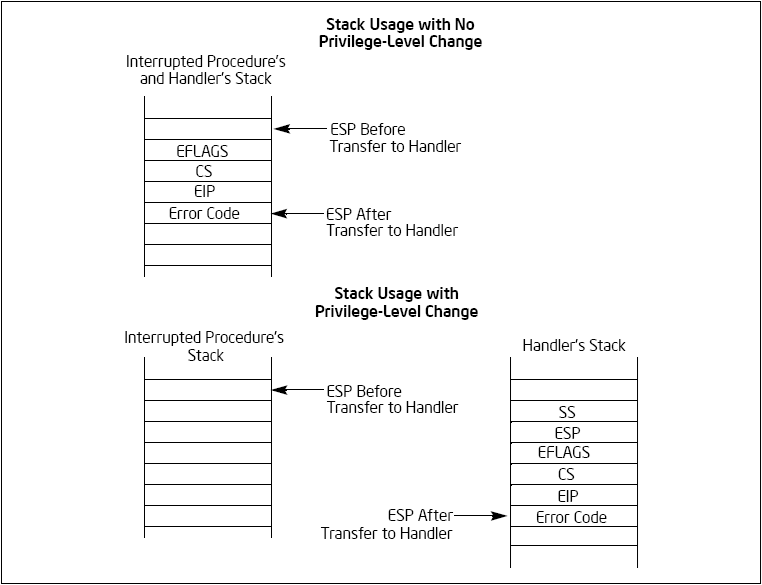
\includegraphics[scale=0.4]{picture/chapt7/interrupt_stack.png}
      \caption{中断发生时CPU保存的现场}
\end{figure}

\par CPU在发生中断的时候是按照上问所描述的过程执行的,那操作系统需要做什么呢?

\par 首先是实现中断处理函数。按照Intel的规定,0~19号中断属于CPU所有\footnote{这些由CPU自身产生的中断也被称之为异常。},而且\allowbreak
第20-31号中断也被Intel保留,所以从32~255号才属于用户自定义中断。虽说是"用户自定义",其实在x86上有些中断按照习惯还是给予了固定\allowbreak
的设备。比如32号是timer中断,33号是键盘中断等等。

\par 中断处理函数怎么实现呢?直接可以进行相关的逻辑处理吗?当然不行了。CPU在中断产生时自动保存了部分的执行现场,但是依旧有很多\allowbreak
寄存器需要我们自己去保护和恢复,下面是CPU保护的寄存器和剩余需要保护的寄存器一起定义的结构体。

\begin{lstlisting}[language = C, caption = include/idt.h]
// 寄存器类型
typedef
struct pt_regs_t {
	uint32_t ds; 		// 用于保存用户的数据段描述符
	uint32_t edi; 		// 从 edi 到 eax 由 pusha 指令压入
	uint32_t esi; 
	uint32_t ebp;
	uint32_t esp;
	uint32_t ebx;
	uint32_t edx;
	uint32_t ecx;
	uint32_t eax;
	uint32_t int_no; 	// 中断号
	uint32_t err_code;  	// 错误代码(有中断错误代码的中断会由CPU压入)
	uint32_t eip; 		// 以下由处理器自动压入
	uint32_t cs; 		
	uint32_t eflags;
	uint32_t useresp;
	uint32_t ss;
} pt_regs;

// 定义中断处理函数指针
typedef void (*interrupt_handler_t)(pt_regs *);

// 注册一个中断处理函数
void register_interrupt_handler(uint8_t n, interrupt_handler_t h);

// 调用中断处理函数
void isr_handler(pt_regs *regs);

// 声明中断处理函数 0 ~ 19 属于 CPU 的异常中断
// ISR:中断服务程序(interrupt service routine)
void isr0(); 		// 0 #DE 除 0 异常 
void isr1(); 		// 1 #DB 调试异常 
void isr2(); 		// 2 NMI 
void isr3(); 		// 3 BP 断点异常 
void isr4(); 		// 4 #OF 溢出 
void isr5(); 		// 5 #BR 对数组的引用超出边界 
void isr6(); 		// 6 #UD 无效或未定义的操作码 
void isr7(); 		// 7 #NM 设备不可用(无数学协处理器) 
void isr8(); 		// 8 #DF 双重故障(有错误代码) 
void isr9(); 		// 9 协处理器跨段操作 
void isr10(); 		// 10 #TS 无效TSS(有错误代码) 
void isr11(); 		// 11 #NP 段不存在(有错误代码) 
void isr12(); 		// 12 #SS 栈错误(有错误代码) 
void isr13(); 		// 13 #GP 常规保护(有错误代码) 
void isr14(); 		// 14 #PF 页故障(有错误代码) 
void isr15(); 		// 15 CPU 保留 
void isr16(); 		// 16 #MF 浮点处理单元错误 
void isr17(); 		// 17 #AC 对齐检查 
void isr18(); 		// 18 #MC 机器检查 
void isr19(); 		// 19 #XM SIMD(单指令多数据)浮点异常

// 20 ~ 31 Intel 保留
void isr20();
void isr21();
void isr22();
void isr23();
void isr24();
void isr25();
void isr26();
void isr27();
void isr28();
void isr29();
void isr30();
void isr31();

// 32 ~ 255 用户自定义异常
void isr255();
\end{lstlisting}

\par 一个很现实的问题是:所有的中断处理函数中,除了CPU本身保护的现场外,其它寄存器的保存和恢复过程都是一样的。所以,\allowbreak
如果在每个中断处理函数中都实现一次显然冗余而且易错。所以我们很自然把原本的中断处理函数逻辑上拆解为三部分,第一部分是\allowbreak
一致的现场保护操作;第二部分是每个中断特有的处理逻辑;第三部分又是一致的现场恢复。

\par 实际上我们把每个中断处理函数拆解为四段,在四个函数里实现。具体的实现如下:

\begin{lstlisting}[language = {[x86masm]Assembler}, caption = idt/idt\_s.s]
; 定义两个构造中断处理函数的宏(有的中断有错误代码,有的没有)
; 用于没有错误代码的中断
%macro ISR_NOERRCODE 1
[GLOBAL isr%1]
isr%1:
	cli                  ; 首先关闭中断
	push 0               ; push 无效的中断错误代码
	push %1              ; push 中断号
	jmp isr_common_stub
%endmacro

; 用于有错误代码的中断
%macro ISR_ERRCODE 1
[GLOBAL isr%1]
isr%1:
	cli                  ; 关闭中断
	push %1              ; push 中断号
	jmp isr_common_stub
%endmacro

; 定义中断处理函数
ISR_NOERRCODE  0 	; 0 #DE 除 0 异常
ISR_NOERRCODE  1 	; 1 #DB 调试异常
ISR_NOERRCODE  2 	; 2 NMI
ISR_NOERRCODE  3 	; 3 BP 断点异常 
ISR_NOERRCODE  4 	; 4 #OF 溢出 
ISR_NOERRCODE  5 	; 5 #BR 对数组的引用超出边界 
ISR_NOERRCODE  6 	; 6 #UD 无效或未定义的操作码 
ISR_NOERRCODE  7 	; 7 #NM 设备不可用(无数学协处理器) 
ISR_ERRCODE    8 	; 8 #DF 双重故障(有错误代码) 
ISR_NOERRCODE  9 	; 9 协处理器跨段操作
ISR_ERRCODE   10 	; 10 #TS 无效TSS(有错误代码) 
ISR_ERRCODE   11 	; 11 #NP 段不存在(有错误代码) 
ISR_ERRCODE   12 	; 12 #SS 栈错误(有错误代码) 
ISR_ERRCODE   13 	; 13 #GP 常规保护(有错误代码) 
ISR_ERRCODE   14 	; 14 #PF 页故障(有错误代码) 
ISR_NOERRCODE 15 	; 15 CPU 保留 
ISR_NOERRCODE 16 	; 16 #MF 浮点处理单元错误 
ISR_ERRCODE   17 	; 17 #AC 对齐检查 
ISR_NOERRCODE 18 	; 18 #MC 机器检查 
ISR_NOERRCODE 19 	; 19 #XM SIMD(单指令多数据)浮点异常

; 20 ~ 31 Intel 保留
ISR_NOERRCODE 20
ISR_NOERRCODE 21
ISR_NOERRCODE 22
ISR_NOERRCODE 23
ISR_NOERRCODE 24
ISR_NOERRCODE 25
ISR_NOERRCODE 26
ISR_NOERRCODE 27
ISR_NOERRCODE 28
ISR_NOERRCODE 29
ISR_NOERRCODE 30
ISR_NOERRCODE 31
; 32 ~ 255 用户自定义
ISR_NOERRCODE 255
\end{lstlisting}

\par 函数执行的开始位置我们自行向栈里压入中断的号码,这是为了识别出中断号码。上面的代码用到了NASM的宏汇编,因为指令结构\allowbreak
是相同的,所以我们可以用宏汇编来生成代码。如果大家对这里有疑问的话,可以参考NASM手册或者直接对生成的内核文件反汇编查看相\allowbreak
关函数的实现。另外还有一点需要说明的是,因为有的中断处理函数会自动压入错误号,而有的不会,这样给我们的清栈造成了麻烦。\allowbreak
所以我们在不会压入错误号的中断的处理函数里手动压入0作为占位,这样方便我们在清理的时候不用分类处理。

\par 以上是中断处理函数的最前一部分,接下来是所有中断处理函数共有的保护现场操作:
\begin{lstlisting}[language = {[x86masm]Assembler}, caption = idt/idt\_s.s]
[GLOBAL isr_common_stub]
[EXTERN isr_handler]
; 中断服务程序
isr_common_stub:
	pusha                    ; Pushes edi, esi, ebp, esp, ebx, edx, ecx, eax
	mov ax, ds
	push eax                ; 保存数据段描述符
	
	mov ax, 0x10            ; 加载内核数据段描述符表
	mov ds, ax
	mov es, ax
	mov fs, ax
	mov gs, ax
	mov ss, ax
	
	push esp		; 此时的 esp 寄存器的值等价于 pt_regs 结构体的指针
	call isr_handler        ; 在 C 语言代码里
	add esp, 4 		; 清除压入的参数
	
	pop ebx                 ; 恢复原来的数据段描述符
	mov ds, bx
	mov es, bx
	mov fs, bx
	mov gs, bx
	mov ss, bx
	
	popa                     ; Pops edi, esi, ebp, esp, ebx, edx, ecx, eax
	add esp, 8               ; 清理栈里的 error code 和 ISR
	iret
.end:
\end{lstlisting}

\par 这里声明了一个外部函数idt\_handler,它的实现如下:
\begin{lstlisting}[language = C, caption = idt/idt.c]
// 调用中断处理函数
void isr_handler(pt_regs *regs)
{
	if (interrupt_handlers[regs->int_no]) {
	      interrupt_handlers[regs->int_no](regs);
	} else {
		printk_color(rc_black, rc_blue, "Unhandled interrupt: %d\n", regs->int_no);
	}
}
\end{lstlisting}

\par 从上面的代码中我们看到,事实上具体的中断处理函数的原型都是 void (pt\_regs *),它们被统一组织放置在了全局的函数指针\allowbreak
数组interrupt\_handers里面。idt\_hanlder函数如判断这个中断函数是否注册,如果注册了会执行该函数,否则打印出Unhandled interrupt和\allowbreak
中断号码。

\par 最后是中断描述符表的创建和和加载函数:
\begin{lstlisting}[language = C, caption = idt/idt.c]
#include "common.h"
#include "string.h"
#include "debug.h"
#include "idt.h"

// 中断描述符表
idt_entry_t idt_entries[256];

// IDTR
idt_ptr_t idt_ptr;

// 中断处理函数的指针数组
interrupt_handler_t interrupt_handlers[256];

// 设置中断描述符
static void idt_set_gate(uint8_t num, uint32_t base, uint16_t sel, uint8_t flags);

// 声明加载 IDTR 的函数
extern void idt_flush(uint32_t);

// 初始化中断描述符表
void init_idt()
{	
	bzero((uint8_t *)&interrupt_handlers, sizeof(interrupt_handler_t) * 256);
	
	idt_ptr.limit = sizeof(idt_entry_t) * 256 - 1;
	idt_ptr.base  = (uint32_t)&idt_entries;
	
	bzero((uint8_t *)&idt_entries, sizeof(idt_entry_t) * 256);

	// 0-32:  用于 CPU 的中断处理
	idt_set_gate( 0, (uint32_t)isr0,  0x08, 0x8E);
	idt_set_gate( 1, (uint32_t)isr1,  0x08, 0x8E);
	idt_set_gate( 2, (uint32_t)isr2,  0x08, 0x8E);
	idt_set_gate( 3, (uint32_t)isr3,  0x08, 0x8E);
	idt_set_gate( 4, (uint32_t)isr4,  0x08, 0x8E);
	idt_set_gate( 5, (uint32_t)isr5,  0x08, 0x8E);
	idt_set_gate( 6, (uint32_t)isr6,  0x08, 0x8E);
	idt_set_gate( 7, (uint32_t)isr7,  0x08, 0x8E);
	idt_set_gate( 8, (uint32_t)isr8,  0x08, 0x8E);
	idt_set_gate( 9, (uint32_t)isr9,  0x08, 0x8E);
	idt_set_gate(10, (uint32_t)isr10, 0x08, 0x8E);
	idt_set_gate(11, (uint32_t)isr11, 0x08, 0x8E);
	idt_set_gate(12, (uint32_t)isr12, 0x08, 0x8E);
	idt_set_gate(13, (uint32_t)isr13, 0x08, 0x8E);
	idt_set_gate(14, (uint32_t)isr14, 0x08, 0x8E);
	idt_set_gate(15, (uint32_t)isr15, 0x08, 0x8E);
	idt_set_gate(16, (uint32_t)isr16, 0x08, 0x8E);
	idt_set_gate(17, (uint32_t)isr17, 0x08, 0x8E);
	idt_set_gate(18, (uint32_t)isr18, 0x08, 0x8E);
	idt_set_gate(19, (uint32_t)isr19, 0x08, 0x8E);
	idt_set_gate(20, (uint32_t)isr20, 0x08, 0x8E);
	idt_set_gate(21, (uint32_t)isr21, 0x08, 0x8E);
	idt_set_gate(22, (uint32_t)isr22, 0x08, 0x8E);
	idt_set_gate(23, (uint32_t)isr23, 0x08, 0x8E);
	idt_set_gate(24, (uint32_t)isr24, 0x08, 0x8E);
	idt_set_gate(25, (uint32_t)isr25, 0x08, 0x8E);
	idt_set_gate(26, (uint32_t)isr26, 0x08, 0x8E);
	idt_set_gate(27, (uint32_t)isr27, 0x08, 0x8E);
	idt_set_gate(28, (uint32_t)isr28, 0x08, 0x8E);
	idt_set_gate(29, (uint32_t)isr29, 0x08, 0x8E);
	idt_set_gate(30, (uint32_t)isr30, 0x08, 0x8E);
	idt_set_gate(31, (uint32_t)isr31, 0x08, 0x8E);

	// 255 将来用于实现系统调用
	idt_set_gate(255, (uint32_t)isr255, 0x08, 0x8E);

	// 更新设置中断描述符表
	idt_flush((uint32_t)&idt_ptr);
}

// 设置中断描述符
static void idt_set_gate(uint8_t num, uint32_t base, uint16_t sel, uint8_t flags)
{
	idt_entries[num].base_lo = base & 0xFFFF;
	idt_entries[num].base_hi = (base >> 16) & 0xFFFF;

	idt_entries[num].sel     = sel;
	idt_entries[num].always0 = 0;

	// 先留下 0x60 这个魔数,以后实现用户态时候
	// 这个与运算可以设置中断门的特权级别为 3
	idt_entries[num].flags = flags;  // | 0x60
}
\end{lstlisting}

\par 加载中断描述符表的函数很简单:
\begin{lstlisting}[language = {[x86masm]Assembler}, caption = idt/idt\_s.s]
[GLOBAL idt_flush]
idt_flush:
	mov eax, [esp+4]  ; 参数存入 eax 寄存器
	lidt [eax]        ; 加载到 IDTR
	ret
.end:
\end{lstlisting}

\par 整理好上面的代码,修改入口函数测试一下中断吧。入口代码修改如下:
\begin{lstlisting}[language = C, caption = init/entry.c]
#include "console.h"
#include "debug.h"
#include "gdt.h"
#include "idt.h"

int kern_entry()
{
	init_debug();
	init_gdt();
	init_idt();

	console_clear();
	printk_color(rc_black, rc_green, "Hello, OS kernel!\n");

	asm volatile ("int $0x3");
	asm volatile ("int $0x4");

	return 0;
}
\end{lstlisting}

\par 编译运行,我们得到了正确的结果:\footnote{当然了,我们没有注册具体的处理函数,所以就打印默认的信息了。}
\begin{figure}[ht]
      \centering
      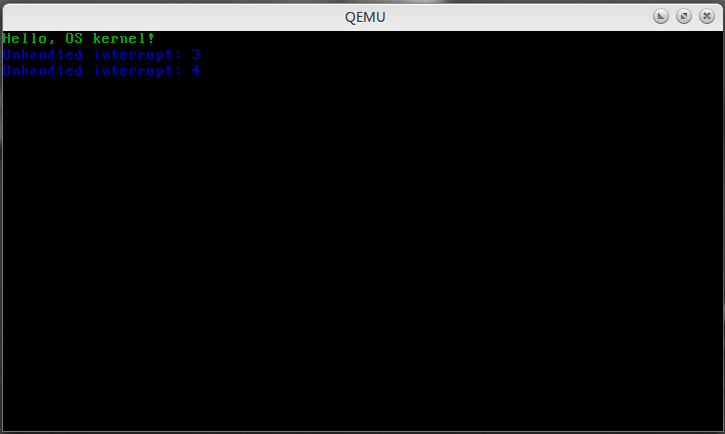
\includegraphics[scale=0.5]{picture/chapt7/interrupt_view.png}
      \caption{中断处理函数的测试}
\end{figure}

% 第8章
% -*- coding: UTF-8 -*-
% hurlex-chapt8.tex
% hurlex 开发文档 第8章内容

\section {完成中断请求和定时器中断}

% 第9章
% -*- coding: UTF-8 -*-
% hurlex-chapt9.tex
% hurlex 开发文档 第9章内容

\section{将内核映射到3G以上的地址空间}

% 第10章
% -*- coding: UTF-8 -*-
% hurlex-chapt10.tex
% hurlex 开发文档 第10章内容

\section {虚拟内存管理的实现}

\par 这章将详细研讨虚拟内存管理的实现。

\par 上一章谈到,虚拟的页面每页占据4KB,按页为单位进行管理。物理内存也被分页管理,按照4KB分为一个个物理页框。虚拟地址到\allowbreak
物理地址通过由页目录和页表组成的二级页表映射,页目录的地址放置在CR3寄存器里。

\par 至此,我们彻底揭开了x86下32位寻址的面纱,下图描述了地址转换的完整过程。

\begin{figure}[H]
      \centering
      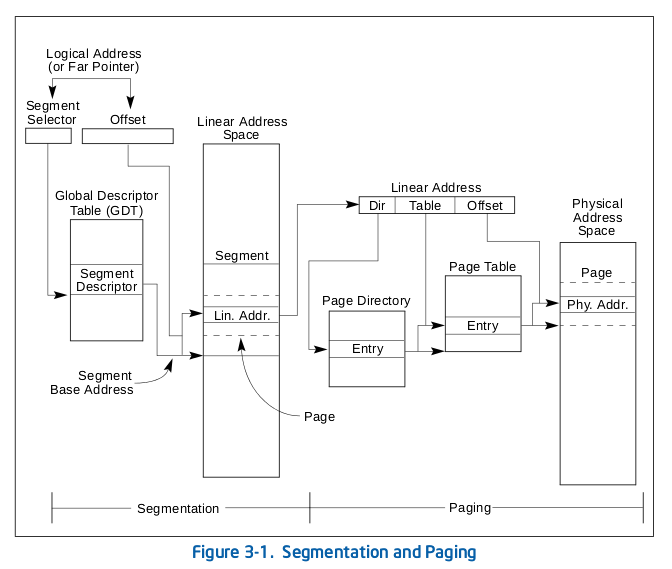
\includegraphics[scale=0.6]{picture/chapt10/ADDR_TRAN.png}
      \caption{段页式转换}
\end{figure}

\par 因为我们使用了Intel平坦模式的内存模型,所以之前的分段机制是被"绕过去"的,所以分页的管理就成了内存管理的核心了。首先是\allowbreak
内核自身地址的映射,Linux采用的是方案是把内核映射到线性地址空间3G以上,而应用程序占据线性地址空间0-3G的位置。我们的内核采取\allowbreak
和Linux内核一样的映射,把物理地址0从虚拟地址0xC0000000(3G)处开始往上映射,因为我们只管理最多512MB的内存,所以3G-4G之间\allowbreak
能完全的映射全部的物理地址。采取这个映射后,物理地址和内核虚拟地址满足以下关系:

\par 物理地址 + 0xC0000000 = 内核虚拟地址

\par 但是采用这个设计的话会给已有的代码带来什么麻烦呢?

\par 我们先引入VMA(Virtual Memory Address)和LMA(Load Memory Address)这两个概念。其中VMA是链接器生成可执行文件时的偏移\allowbreak
计算地址,而LMA是区段所载入内存的实际地址。通常情况下的VMA是等于LMA的。使用以下命令可以查看内核文件的区段信息:
\begin{Verbatim}[frame=single]
    objdump -h hx_kernel
\end{Verbatim}

\par 输出大概是这个样子:

\begin{Verbatim}[frame=single]
hx_kernel:     file format elf32-i386

section:
Idx Name          Size      VMA       LMA       File off  Algn
  0 .text         00003000  00100000  00100000  00000080  2**4
                  CONTENTS, ALLOC, LOAD, READONLY, CODE
  1 .data         00001000  00103000  00103000  00003080  2**2
                  CONTENTS, ALLOC, LOAD, DATA
  2 .bss          00089c64  00104000  00104000  00004080  2**5
                  ALLOC
  3 .stab         0000539c  0018dc64  0018dc64  0008dce4  2**2
                  CONTENTS, ALLOC, LOAD, READONLY, DATA
  4 .stabstr      00002000  00193000  00193000  00093080  2**0
                  CONTENTS, ALLOC, LOAD, READONLY, DATA
\end{Verbatim}

\par 从上面的结果中能看到目前区段的加载地址和虚拟地址都是一样的。按照上面的设计,我们需要修改链接器脚本中各个段的\allowbreak
起始位置。但是简单的把代码段的起始位置设为0xC0100000的话内核一运行就出错。为什么呢?因为GRUB是从1MB处加载内核的,而链\allowbreak
接器是以0xC0100000这个参考地址进行地址重定位的。此时尚未开启虚拟页面映射,运行涉及到寻址的代码肯定就会出错。怎么办呢?\allowbreak
看起来像是一个无解的死循环了。如果GRUB在加载内核之前就能设定好虚拟地址的映射再执行内核多好,或者有一段程序和数据按\allowbreak
照0x100000的地址进行重定位,能帮助我们设置好一个临时的页表,再跳转到内核入口函数多好。前者貌似不可能实现,那后者呢?\allowbreak
答案是肯定的,我们就采用这个方案。

\par GCC提供了这样的扩展机制:允许程序员指定某个函数或者某个变量所存储的区段。同时ld的链接脚本又可以自由定制,所以这个\allowbreak
无解的问题就有了解决方案。用于设置这个临时页表和函数我们指定它存储在.init段,只需要指定该段从0x100000地址开始,\allowbreak
其他的.text和.data等段按照0xC0100000作为起始地址即可。当然这里还有要注意的细节,具体在下面的新链接脚本中可以看。\allowbreak
因为代码变化比较大,所以贴出全部链接器脚本如下:

\begin{lstlisting}[caption = script/kernel.ld]
ENTRY(start)
SECTIONS
{
	PROVIDE( kern_start = 0xC0100000);
	. = 0x100000; 
	.init.text : 
	{
		*(.init.text)
		. = ALIGN(4096);
	}
	.init.data : 
	{
		*(.init.data)
		. = ALIGN(4096);
	}

	. += 0xC0000000;
	.text : AT(ADDR(.text) - 0xC0000000)
	{
		*(.text)
		. = ALIGN(4096);
	}
	.data : AT(ADDR(.data) - 0xC0000000)
	{
		*(.data)
		*(.rodata)
		. = ALIGN(4096);
	}
	.bss : AT(ADDR(.bss) - 0xC0000000)
	{
		*(.bss)
		. = ALIGN(4096);
	}
	.stab : AT(ADDR(.stab) - 0xC0000000)
	{
		*(.stab)
		. = ALIGN(4096);
	}
	.stabstr : AT(ADDR(.stabstr) - 0xC0000000)
	{
		*(.stabstr)
	 	. = ALIGN(4096);
	}
	PROVIDE( kern_end = . );
	
	/DISCARD/ : { *(.comment) *(.eh_frame) }
}
\end{lstlisting}

\par 链接脚本更新之后,之前一些代码也需要做出改动。首先要修改的是入口函数。因为修改的地方略多,所以贴出除声明外完整代码:

\begin{lstlisting}[language = {[x86masm]Assembler}, caption = boot/boot.s]
... ...

[BITS 32]  	; 所有代码以 32-bit 的方式编译

section .init.text 	; 临时代码段从这里开始

; 在代码段的起始位置设置符合 Multiboot 规范的标记

dd MBOOT_HEADER_MAGIC 	; GRUB 会通过这个魔数判断该映像是否支持
dd MBOOT_HEADER_FLAGS   ; GRUB 的一些加载时选项,其详细注释在定义处
dd MBOOT_CHECKSUM       ; 检测数值,其含义在定义处

[GLOBAL start] 		; 内核代码入口,此处提供该声明给 ld 链接器
[GLOBAL mboot_ptr_tmp] 	; 全局的 struct multiboot * 变量
[EXTERN kern_entry] 	; 声明内核 C 代码的入口函数

start:
	cli  				; 此时还没有设置好保护模式的中断处理
					; 所以必须关闭中断
	mov [mboot_ptr_tmp], ebx	; 将 ebx 中存储的指针存入 glb_mboot_ptr 变量
	mov esp, STACK_TOP  		; 设置内核栈地址,按照 multiboot 规范
	and esp, 0FFFFFFF0H		; 栈地址按照 16 字节对齐
	mov ebp, 0 			; 帧指针修改为 0
    
	call kern_entry	; 调用内核入口函数

;-----------------------------------------------------------------------------

section .init.data		; 开启分页前临时的数据段
stack:    times 1024 db 0  	; 这里作为临时内核栈
STACK_TOP equ $-stack-1 	; 内核栈顶,$ 符指代是当前地址

mboot_ptr_tmp: dd 0		; 全局的 multiboot 结构体指针

;-----------------------------------------------------------------------------
\end{lstlisting}

\par 主要的修改是第5行的代码所在段声明和第29行的数据所在段声明,因为此处代码和数据是在参考0x100000(1MB)编址的。\allowbreak
所以在进入分页后需要更换新的内核栈和新的multiboot结构体指针。除此之外,仍就需要指定kern\_entry函数所在区段为.init.text\allowbreak
段,并且在该函数中建立临时页表并跳转到高虚拟地址处的kern\_init函数正式执行,代码如下:

\begin{lstlisting}[language = C, caption = init/entry.c]
#include "console.h"
#include "string.h"
#include "debug.h"
#include "gdt.h"
#include "idt.h"
#include "timer.h"
#include "pmm.h"
#include "vmm.h"

// 内核初始化函数
void kern_init();

// 开启分页机制之后的 Multiboot 数据指针
multiboot_t *glb_mboot_ptr;

// 开启分页机制之后的内核栈
char kern_stack[STACK_SIZE];

// 内核使用的临时页表和页目录
// 该地址必须是页对齐的地址,内存 0-640KB 肯定是空闲的
__attribute__((section(".init.data"))) pgd_t *pgd_tmp  = (pgd_t *)0x1000;
__attribute__((section(".init.data"))) pgd_t *pte_low  = (pgd_t *)0x2000;
__attribute__((section(".init.data"))) pgd_t *pte_hign = (pgd_t *)0x3000;

// 内核入口函数
__attribute__((section(".init.text"))) void kern_entry()
{
	pgd_tmp[0] = (uint32_t)pte_low | PAGE_PRESENT | PAGE_WRITE;
	pgd_tmp[PGD_INDEX(PAGE_OFFSET)] = (uint32_t)pte_hign | PAGE_PRESENT | PAGE_WRITE;

	// 映射内核虚拟地址 4MB 到物理地址的前 4MB
	int i;
	for (i = 0; i < 1024; i++) {
		pte_low[i] = (i << 12) | PAGE_PRESENT | PAGE_WRITE;
	}

	// 映射 0x00000000-0x00400000 的物理地址到虚拟地址 0xC0000000-0xC0400000
	for (i = 0; i < 1024; i++) {
		pte_hign[i] = (i << 12) | PAGE_PRESENT | PAGE_WRITE;
	}
	
	// 设置临时页表
	asm volatile ("mov %0, %%cr3" : : "r" (pgd_tmp));

	uint32_t cr0;

	// 启用分页,将 cr0 寄存器的分页位置为 1 就好
	asm volatile ("mov %%cr0, %0" : "=r" (cr0));
	cr0 |= 0x80000000;
	asm volatile ("mov %0, %%cr0" : : "r" (cr0));
	
	// 切换内核栈
	uint32_t kern_stack_top = ((uint32_t)kern_stack + STACK_SIZE) & 0xFFFFFFF0;
	asm volatile ("mov %0, %%esp\n\t"
			"xor %%ebp, %%ebp" : : "r" (kern_stack_top));

	// 更新全局 multiboot_t 指针
	glb_mboot_ptr = mboot_ptr_tmp + PAGE_OFFSET;

	// 调用内核初始化函数
	kern_init();
}

void kern_init()
{
	init_debug();
	init_gdt();
	init_idt();

	console_clear();
	printk_color(rc_black, rc_green, "Hello, OS kernel!\n\n");

	init_timer(200);

	// 开启中断
	// asm volatile ("sti");

	printk("kernel in memory start: 0x%08X\n", kern_start);
	printk("kernel in memory end:   0x%08X\n", kern_end);
	printk("kernel in memory used:   %d KB\n\n", (kern_end - kern_start) / 1024);
	
	show_memory_map();
	init_pmm();

	printk_color(rc_black, rc_red, "\nThe Count of Physical Memory Page is: %u\n\n", phy_page_count);

	uint32_t allc_addr = NULL;
	printk_color(rc_black, rc_light_brown, "Test Physical Memory Alloc :\n");
	allc_addr = pmm_alloc_page();
	printk_color(rc_black, rc_light_brown, "Alloc Physical Addr: 0x%08X\n", allc_addr);
	allc_addr = pmm_alloc_page();
	printk_color(rc_black, rc_light_brown, "Alloc Physical Addr: 0x%08X\n", allc_addr);
	allc_addr = pmm_alloc_page();
	printk_color(rc_black, rc_light_brown, "Alloc Physical Addr: 0x%08X\n", allc_addr);
	allc_addr = pmm_alloc_page();
	printk_color(rc_black, rc_light_brown, "Alloc Physical Addr: 0x%08X\n", allc_addr);

	while (1) {
		asm volatile ("hlt");
	}
}
\end{lstlisting}

\par 代码中的 \_\_attribute\_\_((section(".init.data"))) 是GCC编译器的扩展功能,用来指定变量或者函数的存储区段。我们\allowbreak
使用了1MB以下地址空间中的12KB来暂时放置临时页表。除此之外,入口函数中除了映射0xC0000000(3G)开始的4MB地址到物理内存\allowbreak
0-4MB之外,我们依旧把虚拟地址的0-4MB映射到了物理地址的同样位置。为什么呢?因为在代码48-50行一旦将CR0寄存器最高位置为1\allowbreak
的话,CPU立即就会进入分页机制去运行,此时所有的寻址都会按照分页机制的原则去进行,而kern\_entry函数本身是按照1MB起始地址\allowbreak
生成的虚拟地址,如果不映射低端的虚拟地址的话,kern\_entry开启分页之后的代码访问就会出错。而最终离开了这个入口函数,进入\allowbreak
内核初始化函数kern\_init的时候,已经处于高端虚拟地址的区域。所以在新的页表里不再需要低端的映射也可以正常寻址了。

\par 别忘了要更新multiboot.h的声明:

\begin{lstlisting}[language = C, caption = include/multiboot.h]
// 声明全局的 multiboot_t * 指针
// 内核未建立分页机制前暂存的指针
extern multiboot_t *mboot_ptr_tmp;

// 内核页表建立后的指针
extern multiboot_t *glb_mboot_ptr;

\end{lstlisting}

\par 另外还需要修改文本模式下显存的起始位置,原先的地址0xB8000此时需要加上偏移地址0xC0000000才可以在分页模式下正常访问到。

\begin{lstlisting}[language = C, caption = drivers/console.c]
... ...
// VGA 的显示缓冲的起点是 0xB8000
static uint16_t *video_memory = (uint16_t *)(0xB8000 + PAGE_OFFSET);
... ...
\end{lstlisting}

\par 最后是实现虚拟内存管理的初始化了,这个函数将建立正式的内核页表并进行切换。同时还有进行地址映射和解除映射的函数实现:

\begin{lstlisting}[language = C, caption = mm/vmm.c]
#include "idt.h"
#include "string.h"
#include "debug.h"
#include "vmm.h"
#include "pmm.h"

// 内核页目录区域
pgd_t pgd_kern[PGD_SIZE] __attribute__ ((aligned(PAGE_SIZE)));

// 内核页表区域
static pte_t pte_kern[PTE_COUNT][PTE_SIZE] __attribute__ ((aligned(PAGE_SIZE)));

void init_vmm()
{
	// 0xC0000000 这个地址在页目录的索引
	uint32_t kern_pte_first_idx = PGD_INDEX(PAGE_OFFSET);
	
	uint32_t i, j;
	for (i = kern_pte_first_idx, j = 0; i < PTE_COUNT + kern_pte_first_idx; i++, j++) {
		// 此处是内核虚拟地址,MMU 需要物理地址,所以减去偏移,下同
		pgd_kern[i] = ((uint32_t)pte_kern[j] - PAGE_OFFSET) | PAGE_PRESENT | PAGE_WRITE;
	}

	uint32_t *pte = (uint32_t *)pte_kern;
	// 不映射第 0 页,便于跟踪 NULL 指针
	for (i = 1; i < PTE_COUNT * PTE_SIZE; i++) {
		pte[i] = (i << 12) | PAGE_PRESENT | PAGE_WRITE;
	}

	uint32_t pgd_kern_phy_addr = (uint32_t)pgd_kern - PAGE_OFFSET;

	// 注册页错误中断的处理函数 ( 14 是页故障的中断号 )
	register_interrupt_handler(14, &page_fault);

	switch_pgd(pgd_kern_phy_addr);
}

void switch_pgd(uint32_t pd)
{
	asm volatile ("mov %0, %%cr3" : : "r" (pd));
}

void map(pgd_t *pgd_now, uint32_t va, uint32_t pa, uint32_t flags)
{ 	
	uint32_t pgd_idx = PGD_INDEX(va);
	uint32_t pte_idx = PTE_INDEX(va); 
	
	pte_t *pte = (pte_t *)(pgd_now[pgd_idx] & PAGE_MASK);
	if (!pte) {
		pte = (pte_t *)pmm_alloc_page();
		pgd_now[pgd_idx] = (uint32_t)pte | PAGE_PRESENT | PAGE_WRITE;

		// 转换到内核线性地址并清 0
		pte = (pte_t *)((uint32_t)pte + PAGE_OFFSET);
		bzero(pte, PAGE_SIZE);
	} else {
		// 转换到内核线性地址
		pte = (pte_t *)((uint32_t)pte + PAGE_OFFSET);
	}

	pte[pte_idx] = (pa & PAGE_MASK) | flags;

	// 通知 CPU 更新页表缓存
	asm volatile ("invlpg (%0)" : : "a" (va));
}

void unmap(pgd_t *pgd_now, uint32_t va)
{
	uint32_t pgd_idx = PGD_INDEX(va);
	uint32_t pte_idx = PTE_INDEX(va);

	pte_t *pte = (pte_t *)(pgd_now[pgd_idx] & PAGE_MASK);

	if (!pte) {
		return;
	}

	// 转换到内核线性地址
	pte = (pte_t *)((uint32_t)pte + PAGE_OFFSET);

	pte[pte_idx] = 0;

	// 通知 CPU 更新页表缓存
	asm volatile ("invlpg (%0)" : : "a" (va));
}

uint32_t get_mapping(pgd_t *pgd_now, uint32_t va, uint32_t *pa)
{
	uint32_t pgd_idx = PGD_INDEX(va);
	uint32_t pte_idx = PTE_INDEX(va);

	pte_t *pte = (pte_t *)(pgd_now[pgd_idx] & PAGE_MASK);
	if (!pte) {
	      return 0;
	}
	
	// 转换到内核线性地址
	pte = (pte_t *)((uint32_t)pte + PAGE_OFFSET);

	// 如果地址有效而且指针不为NULL,则返回地址
	if (pte[pte_idx] != 0 && pa) {
		 *pa = pte[pte_idx] & PAGE_MASK;
		return 1;
	}

	return 0;
}
\end{lstlisting}

\par 需要注意的是Intel规定页表和页目录得的起始位置必须是页对齐的,\_\_attribute\_\_ ((aligned(PAGE\_SIZE))) 是GCC的扩展\allowbreak
指令,功能是使得变量的起始地址按照某个数值对齐,所以我们轻轻松松的就解决了这个难题。

\par 上面代码对应的头文件如下:

\begin{lstlisting}[language = C, caption = include/vmm.h]
#ifndef INCLUDE_VMM_H
#define INCLUDE_VMM_H

#include "types.h"
#include "idt.h"
#include "vmm.h"

// 内核的偏移地址
#define PAGE_OFFSET 	0xC0000000

/**
 * P--位0是存在(Present)标志,用于指明表项对地址转换是否有效。P=1表示有效;P=0表示无效。
 * 在页转换过程中,如果说涉及的页目录或页表的表项无效,则会导致一个异常。
 * 如果P=0,那么除表示表项无效外,其余位可供程序自由使用。
 * 例如,操作系统可以使用这些位来保存已存储在磁盘上的页面的序号。
 */
#define PAGE_PRESENT 	0x1

/** 
 * R/W--位1是读/写(Read/Write)标志。如果等于1,表示页面可以被读、写或执行。
 * 如果为0,表示页面只读或可执行。
 * 当处理器运行在超级用户特权级(级别0、1或2)时,则R/W位不起作用。
 * 页目录项中的R/W位对其所映射的所有页面起作用。
 */
#define PAGE_WRITE 	0x2

/**
 * U/S--位2是用户/超级用户(User/Supervisor)标志。
 * 如果为1,那么运行在任何特权级上的程序都可以访问该页面。
 * 如果为0,那么页面只能被运行在超级用户特权级(0、1或2)上的程序访问。
 * 页目录项中的U/S位对其所映射的所有页面起作用。
 */
#define PAGE_USER 	0x4

// 虚拟分页大小
#define PAGE_SIZE 	4096

// 页掩码,用于 4KB 对齐
#define PAGE_MASK      0xFFFFF000

// 获取一个地址的页目录项
#define PGD_INDEX(x) (((x) >> 22) & 0x3FF)

// 获取一个地址的页表项
#define PTE_INDEX(x) (((x) >> 12) & 0x3FF)

// 获取一个地址的页內偏移
#define OFFSET_INDEX(x) ((x) & 0xFFF)

// 页目录数据类型
typedef uint32_t pgd_t;

// 页表数据类型
typedef uint32_t pte_t;

// 页表成员数
#define PGD_SIZE (PAGE_SIZE/sizeof(pte_t))

// 页表成员数
#define PTE_SIZE (PAGE_SIZE/sizeof(uint32_t))

// 映射 512MB 内存所需要的页表数
#define PTE_COUNT 128

// 内核页目录区域
extern pgd_t pgd_kern[PGD_SIZE];

// 初始化虚拟内存管理
void init_vmm();

// 更换当前的页目录
void switch_pgd(uint32_t pd);

// 使用 flags 指出的页权限,把物理地址 pa 映射到虚拟地址 va
void map(pgd_t *pgd_now, uint32_t va, uint32_t pa, uint32_t flags);

// 取消虚拟地址 va 的物理映射
void unmap(pgd_t *pgd_now, uint32_t va);

// 如果虚拟地址 va 映射到物理地址则返回 1
// 同时如果 pa 不是空指针则把物理地址写入 pa 参数
uint32_t get_mapping(pgd_t *pgd_now, uint32_t va, uint32_t *pa);

// 页错误中断的函数处理
void page_fault(pt_regs *regs);

#endif 	// INCLUDE_VMM_H
\end{lstlisting}

\par 整理好代码后进行编译,再用objdump查看可执行文件的段表,输出大致如下:

\begin{Verbatim}[frame=single]
hx_kernel:     file format elf32-i386

section:
Idx Name          Size      VMA       LMA       File off  Algn
  0 .init.text    00001000  00100000  00100000  00000094  2**0
                  CONTENTS, ALLOC, LOAD, READONLY, CODE
  1 .init.data    00001000  00101000  00101000  00001094  2**2
                  CONTENTS, ALLOC, LOAD, DATA
  2 .text         00003000  c0102000  00102000  00003000  2**4
                  CONTENTS, ALLOC, LOAD, READONLY, CODE
  3 .data         00001000  c0105000  00105000  00006000  2**2
                  CONTENTS, ALLOC, LOAD, DATA
  4 .bss          00105000  c0106000  00106000  00007000  2**12
                  ALLOC
  5 .stab         00005000  c020b000  0020b000  0010c000  2**2
                  CONTENTS, ALLOC, LOAD, READONLY, DATA
  6 .stabstr      00002000  c0210000  00210000  00111000  2**0
                  CONTENTS, ALLOC, LOAD, READONLY, DATA
\end{Verbatim}

\par 我们看到前两个区段和以前的输出类似,但是后面区段的VMA已经变成了加上了0xC0000000偏移的地址了。如果运行后能看到和\allowbreak
上一章相同的输出结果就没有问题了。如果你得不到正确的结果,那就自己动手调试吧。


% 第11章
% -*- coding: UTF-8 -*-
% hurlex-chapt11.tex
% hurlex 开发文档 第11章内容

\section {内核堆管理的实现}

\par 前几章实现了内存的简单管理,但是目前的内存分配是按页为单位的,这样在需要分配小内存的时候比较容易造成内部碎片。\allowbreak
这章我们来实现内核的堆管理算法,目的是为了小内存的分配。除了简单的分配内存之外,还需要考虑在内存释放的时候,对连续\allowbreak
的内存进行合并。并且堆要实现在空闲内存过多的时候把物理页释放给物理内存管理模块。

\par 关于堆的实现有很多种,我们选择最简单的侵入式链表管理方法。如果你觉得可以胜任更好的算法完全可以自由发挥,而且之前\allowbreak
的物理内存管理算法完全可以实现为伙伴系统。不过为了照顾大多数读者,我们选择简单的方式实现。当然,通过简单得的算法熟悉了\allowbreak
物理的机制之后,完全可以抛开这些简单实现,去实现更好的算法。

\par 首先,在每一个申请的内存块之前插入一个描述当前内存块的结构体。结构体定义以及相关的函数声明如下:

\begin{lstlisting}[language = C, caption = include/heap.h]
#ifndef INCLUDE_HEAP_H_
#define INCLUDE_HEAP_H_

#include "types.h"

// 堆起始地址
#define HEAP_START 0xE0000000

// 内存块管理结构
typedef
struct header {
	struct header *prev; 	// 前后内存块管理结构指针
	struct header *next;
	uint32_t allocated : 1;	// 该内存块是否已经被申请
	uint32_t length : 31; 	// 当前内存块的长度
} header_t;

// 初始化堆
void init_heap();

// 内存申请
void *kmalloc(uint32_t len);

// 内存释放
void kfree(void *p);

// 测试内核堆申请释放
void test_heap();

#endif 	// INCLUDE_HEAP_H_
\end{lstlisting}

\par 结构体的定义里使用了C语言的位域定义,因为表示这块内存有没有被使用只需要1个bit就可以,这样节省内存。这里定义的\allowbreak
堆的函数形式很简单,就不详细解释了。需要注意的是这里定义了虚拟堆起始地址为0xE0000000,它是内核页表没有使用的空闲区域。

\par 接下来是具体实现。除了以上的外部接口函数,还需要在实现文件里声明以下内部函数:

\begin{lstlisting}[language = C, caption = mm/heap.c]
#include "debug.h"
#include "pmm.h"
#include "vmm.h"
#include "heap.h"

// 申请内存块
static void alloc_chunk(uint32_t start, uint32_t len);

// 释放内存块
static void free_chunk(header_t *chunk);

// 切分内存块
static void split_chunk(header_t *chunk, uint32_t len);

// 合并内存块
static void glue_chunk(header_t *chunk);

static uint32_t heap_max = HEAP_START;

// 内存块管理头指针
static header_t *heap_first;
\end{lstlisting}

\par 这些内部函数只在堆的内部被调用,所以被声明为static,我们之前也强调过,不需要向外部暴露的函数最好用static限制其作用域。\allowbreak
我们直接贴出相关函数的实现:

\begin{lstlisting}[language = C, caption = mm/heap.c]
... ...

void init_heap()
{
	heap_first = 0;
}

void *kmalloc(uint32_t len)
{
	// 所有申请的内存长度加上管理头的长度
	// 因为在内存申请和释放的时候要通过该结构去管理
	len += sizeof(header_t);

	header_t *cur_header = heap_first;
	header_t *prev_header = 0;

	while (cur_header) {
		// 如果当前内存块没有被申请过而且长度大于待申请的块
		if (cur_header->allocated == 0 && cur_header->length >= len) {
			// 按照当前长度切割内存
			split_chunk(cur_header, len);
			cur_header->allocated = 1;
			// 返回的时候必须将指针挪到管理结构之后
			return (void *)((uint32_t)cur_header + sizeof(header_t));
		}
		// 逐次推移指针
		prev_header = cur_header;
		cur_header = cur_header->next;
	}

	uint32_t chunk_start;

	// 第一次执行该函数则初始化内存块起始位置
	// 之后根据当前指针加上申请的长度即可
	if (prev_header) {
		chunk_start = (uint32_t)prev_header + prev_header->length;
	} else {
		chunk_start = HEAP_START;
		heap_first = (header_t *)chunk_start;
	}

	// 检查是否需要申请内存页
	alloc_chunk(chunk_start, len);
	cur_header = (header_t *)chunk_start;
	cur_header->prev = prev_header;
	cur_header->next = 0;
	cur_header->allocated = 1;
	cur_header->length = len;
	
	if (prev_header) {
		prev_header->next = cur_header;
	}

	return (void*)(chunk_start + sizeof(header_t));
}

void kfree(void *p)
{
	// 指针回退到管理结构,并将已使用标记置 0
	header_t *header = (header_t*)((uint32_t)p - sizeof(header_t));
	header->allocated = 0;

	// 粘合内存块
	glue_chunk(header);
}

void alloc_chunk(uint32_t start, uint32_t len)
{
	// 如果当前堆的位置已经到达界限则申请内存页
	// 必须循环申请内存页直到有到足够的可用内存
	while (start + len > heap_max) {
		uint32_t page = pmm_alloc_page();
		map(pgd_kern, heap_max, page, PAGE_PRESENT | PAGE_WRITE);
		heap_max += PAGE_SIZE;
	}
}

void free_chunk(header_t *chunk)
{
	if (chunk->prev == 0) {
		heap_first = 0;
	} else {
		chunk->prev->next = 0;
	}

	// 空闲的内存超过 1 页的话就释放掉
	while ((heap_max - PAGE_SIZE) >= (uint32_t)chunk) {
		heap_max -= PAGE_SIZE;
		uint32_t page;
		get_mapping(pgd_kern, heap_max, &page);
		unmap(pgd_kern, heap_max);
		pmm_free_page(page);
	}
}

void split_chunk(header_t *chunk, uint32_t len)
{
	// 切分内存块之前得保证之后的剩余内存至少容纳一个内存管理块的大小
	if (chunk->length - len > sizeof (header_t)) {
		header_t *newchunk = (header_t *)((uint32_t)chunk + chunk->length);
		newchunk->prev = chunk;
		newchunk->next = chunk->next;
		newchunk->allocated = 0;
		newchunk->length = chunk->length - len;

		chunk->next = newchunk;
		chunk->length = len;
	}
}

void glue_chunk(header_t *chunk)
{
	// 如果该内存块前面有链内存块且未被使用则拼合
	if (chunk->next && chunk->next->allocated == 0) {
		chunk->length = chunk->length + chunk->next->length;
		if (chunk->next->next) {
			chunk->next->next->prev = chunk;
		}
		chunk->next = chunk->next->next;
	}

	if (chunk->prev && chunk->prev->allocated == 0) {
		chunk->prev->length = chunk->prev->length + chunk->length;
		chunk->prev->next = chunk->next;
		if (chunk->next) {
			chunk->next->prev = chunk->prev;
		}
		chunk = chunk->prev;
	}

	// 假如该内存后面没有链表内存块了直接释放掉
	if (chunk->next == 0) {
		free_chunk(chunk);
	}
}
... ...
\end{lstlisting}

\par 这里的代码都很简单,只是链表的简单运用。需要注意的是映射和解除映射并释放的函数。如果理解起来有困难的话,建议你在\allowbreak
调试模式下在纸上画一画,这样很容易理解。\footnote{这里的代码基本上来自Jamesm先生的实现,不过Jamesm先生的实现隐藏了比较多\allowbreak
的BUG,我也是在纸上画过之后才找出的BUG。}

\par 最后添加一个简单的测试函数:

\begin{lstlisting}[language = C, caption = mm/heap.c]
void test_heap()
{
	printk_color(rc_black, rc_magenta, "Test kmalloc() && kfree() now ...\n\n");

	void *addr1 = kmalloc(50);
	printk("kmalloc    50 byte in 0x%X\n", addr1);
	void *addr2 = kmalloc(500);
	printk("kmalloc   500 byte in 0x%X\n", addr2);
	void *addr3 = kmalloc(5000);
	printk("kmalloc  5000 byte in 0x%X\n", addr3);
	void *addr4 = kmalloc(50000);
	printk("kmalloc 50000 byte in 0x%X\n\n", addr4);

	printk("free mem in 0x%X\n", addr1);
	kfree(addr1);
	printk("free mem in 0x%X\n", addr2);
	kfree(addr2);
	printk("free mem in 0x%X\n", addr3);
	kfree(addr3);
	printk("free mem in 0x%X\n\n", addr4);
	kfree(addr4);
}
\end{lstlisting}

\par 最后自然是测试了。在内核的初始化函数里加上堆的相关头文件并且调用初始化和测试函数,输出如下:

\begin{figure}[ht]
      \centering
      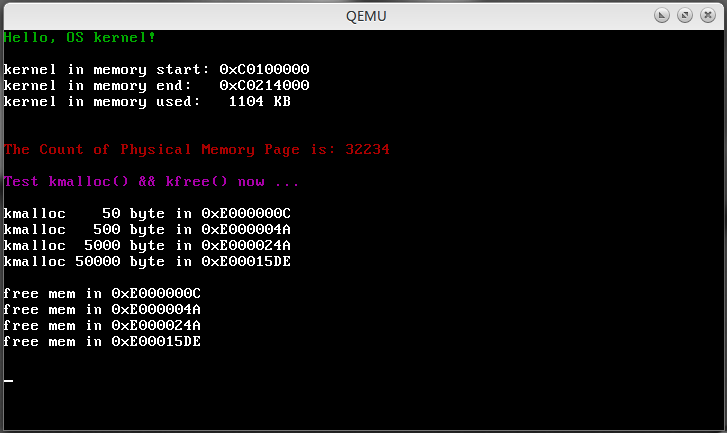
\includegraphics[scale=0.6]{picture/chapt11/HEAP_TEST.png}
      \caption{内核堆管理函数的测试}
\end{figure}

\par OK,任务完成!

% 第12章
% -*- coding: UTF-8 -*-
% hurlex-chapt12.tex
% hurlex 开发文档 第12章内容

\section {内核线程的创建与切换}

\par 这章讨论内核线程的创建与切换。

\par 首先给出这里内核线程的含义,此处的内核线程作为运行在内核态的一个逻辑执行流,拥有私有的栈空间。但是除了这个私有的栈之外,\allowbreak
不拥有其它的资源。所有的内核线程拥有相同的页表,共享所有的全局数据。

\par Intel的x86CPU提供任务切换机制是使用TSS段进行切换,这么做比较繁琐且效率较低,现代的OS都不会完全采用硬件切换机制。本章所\allowbreak
阐述的任务切换只发生在内核态,不涉及特权级的转移过程,所以可以完全由硬件实现。而且这种实现用在用户级的线程库中亦可,大家有兴趣\allowbreak
的话可以仿照这个思路实现用户级线程库。

\par 任务的切换必然涉及到现场的保护与恢复,所以就必然需要一个数据结构来保存这些现场信息。这个数据结构中一般也会放置任务相关的\allowbreak
一些信息并且以链表之类的方式组织起来,这个结构被称之为PCB(Process Control Block)或者TCB(Task Control Block)。相关定义如下:

\begin{lstlisting}[language = C, caption = include/task.h]
#ifndef INCLUDE_TASK_H_
#define INCLUDE_TASK_H_

#include "types.h"
#include "pmm.h"
#include "vmm.h"

// 进程状态描述
typedef
enum task_state {
	TASK_UNINIT = 0, 	// 未初始化
	TASK_SLEEPING = 1, 	// 睡眠中
	TASK_RUNNABLE = 2, 	// 可运行(也许正在运行)
	TASK_ZOMBIE = 3, 	// 僵尸状态
} task_state;

// 内核线程的上下文切换保存的信息
struct context {
	uint32_t esp;
	uint32_t ebp;
	uint32_t ebx;
	uint32_t esi;
	uint32_t edi;
	uint32_t eflags;
};

// 进程内存地址结构
struct mm_struct {
	pgd_t *pgd_dir; 	// 进程页表
};

// 进程控制块 PCB 
struct task_struct {
	volatile task_state state; 	// 进程当前状态
	pid_t 	 pid; 			// 进程标识符
	void  	*stack; 		// 进程的内核栈地址
	struct mm_struct *mm; 		// 当前进程的内存地址映像
	struct context context; 	// 进程切换需要的上下文信息
	struct task_struct *next; 	// 链表指针
};

// 全局 pid 值
extern pid_t now_pid;

// 内核线程创建
int32_t kernel_thread(int (*fn)(void *), void *arg);

// 线程退出函数
void kthread_exit();

#endif 	// INCLUDE_TASK_H_
\end{lstlisting}

\par 除了描述每一个任务信息的结构,还需要将这些结构组织起来并且引入调度机制。相关的头文件和定义如下:

\begin{lstlisting}[language = C, caption = include/sched.h]
#ifndef INCLUDE_SCHEDULER_H_
#define INCLUDE_SCHEDULER_H_

#include "task.h"

// 可调度进程链表
extern struct task_struct *running_proc_head;

// 等待进程链表
extern struct task_struct *wait_proc_head;

// 当前运行的任务
extern struct task_struct *current;

// 初始化任务调度
void init_sched();

// 任务调度
void schedule();

// 任务切换准备
void change_task_to(struct task_struct *next);

// 任务切换
void switch_to(struct context *prev, struct context *next);

#endif 	// INCLUDE_SCHEDULER_H_
\end{lstlisting}

\par 本章中不会采用复杂的调度策略,操作系统理论中各种调度算法都不会在这里实现。本章主要目的是说明白任务切换的原理。所以任务\allowbreak
组织的方式就是一个单向循环链表,调度程序每次选择当前任务的下一个任务运行。如果你有兴趣,可以自己实现更好的调度算法。大家完全\allowbreak
可以在PCB里增加新的数据成员,实现带有优先级的任务切换机制。

\par 在进行任务切换之前,内核原先的执行流还没有一个结构来保存其信息,所以需要在初始化调度之前给原始的执行流创建PCB信息。\allowbreak
这里模仿Linux内核早期的做法,将PCB放置在线程栈的最低处。初始化的代码如下:

\begin{lstlisting}[language = C, caption = kernel/sched/sched.c]
#include "sched.h"
#include "heap.h"
#include "debug.h"

// 可调度进程链表
struct task_struct *running_proc_head = NULL;

// 等待进程链表
struct task_struct *wait_proc_head = NULL;

// 当前运行的任务
struct task_struct *current = NULL;

void init_sched()
{
	// 为当前执行流创建信息结构体 该结构位于当前执行流的栈最低端
	current = (struct task_struct *)(kern_stack_top - STACK_SIZE);

	current->state = TASK_RUNNABLE;
	current->pid = now_pid++;
	current->stack = current; 	// 该成员指向栈低地址
	current->mm = NULL; 		// 内核线程不需要该成员

	// 单向循环链表
	current->next = current;

	running_proc_head = current;
}
\end{lstlisting}

\par 调度函数很容易理解,每次都返回当前任务的下一个任务。代码如下:
\footnote{这里的调度函数留给大家自由发挥,去自由实现各种高端的调度算法。}

\begin{lstlisting}[language = C, caption = include/sched.h]
void schedule()
{
	if (current) {
		change_task_to(current->next);
	}
}

void change_task_to(struct task_struct *next)
{
	if (current != next) {
		struct task_struct *prev = current;
		current = next;
		switch_to(&(prev->context), &(current->context));
	}
}
\end{lstlisting}

\par 具体的切换操作由汇编实现,分别是保存当前任务的执行上下文和切换到下一个任务去。代码如下:

\begin{lstlisting}[language = {[x86masm]Assembler}, caption = kernel/sched/switch\_to.s]
[global switch_to]

; 具体的线程切换操作,重点在于寄存器的保存与恢复
switch_to:
        mov eax, [esp+4]

        mov [eax+0],  esp
        mov [eax+4],  ebp
        mov [eax+8],  ebx
        mov [eax+12], esi
        mov [eax+16], edi
        pushf
        pop ecx
        mov [eax+20], ecx

        mov eax, [esp+8]

        mov esp, [eax+0]
        mov ebp, [eax+4]
        mov ebx, [eax+8]
        mov esi, [eax+12]
        mov edi, [eax+16]
        mov eax, [eax+20]
        push eax
        popf
 	
        ret
\end{lstlisting}

\par 经过上面的铺垫,重头戏就是接下来的切换了。内核线程的创建和退出函数的实现如下:

\begin{lstlisting}[language = C, caption = include/task.h]
#include "gdt.h"
#include "pmm.h"
#include "vmm.h"
#include "heap.h"
#include "task.h"
#include "sched.h"
#include "string.h"
#include "debug.h"

// 全局 pid 值
pid_t now_pid = 0;

// 内核线程创建
int32_t kernel_thread(int (*fn)(void *), void *arg)
{
	struct task_struct *new_task = (struct task_struct *)kmalloc(STACK_SIZE);
	assert(new_task != NULL, "kern_thread: kmalloc error");

	// 将栈低端结构信息初始化为 0 
	bzero(new_task, sizeof(struct task_struct));

	new_task->state = TASK_RUNNABLE;
	new_task->stack = current;
	new_task->pid = now_pid++;
	new_task->mm = NULL;

	uint32_t *stack_top = (uint32_t *)((uint32_t)new_task + STACK_SIZE);

	*(--stack_top) = (uint32_t)arg;
	*(--stack_top) = (uint32_t)kthread_exit;
	*(--stack_top) = (uint32_t)fn;

	new_task->context.esp = (uint32_t)new_task + STACK_SIZE - sizeof(uint32_t) * 3;

	// 设置新任务的标志寄存器未屏蔽中断,很重要
	new_task->context.eflags = 0x200;
	new_task->next = running_proc_head;
	
	// 找到当前进任务队列,插入到末尾
	struct task_struct *tail = running_proc_head;
	assert(tail != NULL, "Must init sched!");

	while (tail->next != running_proc_head) {
		tail = tail->next;
	}
	tail->next = new_task;

	return new_task->pid;
}

void kthread_exit()
{
	register uint32_t val asm ("eax");

	printk("Thread exited with value %d\n", val);

	while (1);
}

\end{lstlisting}

\par 内核退出函数在这里只实现了简陋的一部分,标准做法是将退出线程的PCB结构转移到不可调度链表去,等待其他线程join后再\allowbreak
清理结构。这个留给大家自由实现吧,可以自由发散思维去做。

\par 这里的内核线程的创建和切换过程可能有些晦涩,其切换的重点在于switch\_to函数最后的ret指令。在ret指令返回之前,由于之前的\allowbreak
执行现场已经被切换,特别是esp指针指向的栈被切换了,所以ret指令弹出的返回地址自然就变成了另一个执行流之前调用任务切换函数\allowbreak
之前保存的返回地址了。kernel\_thread函数便是通过构造出这样一个切换后可以弹出执行地址的初始栈来实现的。
\footnote{如果理解起来依旧有困难的话不妨在纸上画画调用栈,这样比较好理解。}

\par 解决了所有切换的问题之后,剩下的只是时间片的问题了。可能大家已经想到了,这个调度函数最终是要由timer中断函数来执行的。\allowbreak
我们修改timer中断的处理函数如下:

\begin{lstlisting}[language = C, caption = drivers/timer.c]
void timer_callback(pt_regs *regs)
{
	schedule();
}
\end{lstlisting}

\par 在定时器初始化之后,我们开启INTR中断。此时timer中断会按照之前设定好的工作频率来执行调度任务。

\par 我们在初始化函数里测试下,代码如下:

\begin{lstlisting}[language = C, caption = init/entry.c]

... ...

int flag = 0;

int thread(void *arg)
{
	while (1) {
		if (flag == 1) {
			printk_color(rc_black, rc_green, "B");
			flag = 0;
		}
	}

	return 0;
}

void kern_init()
{
	init_debug();
	init_gdt();
	init_idt();

	console_clear();
	printk_color(rc_black, rc_green, "Hello, OS kernel!\n\n");

	init_timer(200);

	printk("kernel in memory start: 0x%08X\n", kern_start);
	printk("kernel in memory end:   0x%08X\n", kern_end);
	printk("kernel in memory used:   %d KB\n\n", (kern_end - kern_start) / 1024);
	
	// show_memory_map();
	init_pmm();
	init_vmm();
	init_heap();

	printk_color(rc_black, rc_red, "\nThe Count of Physical Memory Page is: %u\n\n", phy_page_count);
	test_heap();

	init_sched();

	kernel_thread(thread, NULL);

	// 开启中断
	enable_intr();

	while (1) {
		if (flag == 0) {
			printk_color(rc_black, rc_red, "A");
			flag = 1;
		}
	}

	while (1) {
		asm volatile ("hlt");
	}
}
\end{lstlisting}

\par 编译运行后,我们看到了完美交替输出的A和B,如图所示:

\begin{figure}[ht]
      \centering
      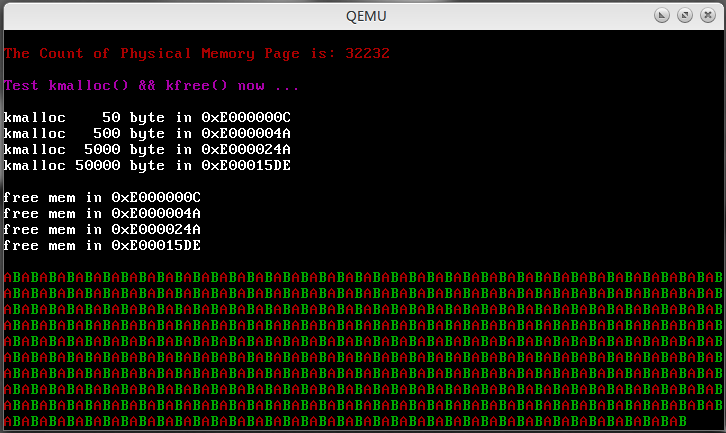
\includegraphics[scale=0.6]{picture/chapt12/KTHREAD.png}
      \caption{测试内核线程切换}
\end{figure}


% 第13章
% -*- coding: UTF-8 -*-
% hurlex-chapt14.tex
% hurlex 开发文档 第14章内容

\section {从内核态迈向用户态}

% 第14章
% -*- coding: UTF-8 -*-
% hurlex-chapt15.tex
% hurlex 开发文档 第15章内容

\section{系统调用的简单实现}

% 第15章
% -*- coding: UTF-8 -*-
% hurlex-chapt15.tex
% hurlex 开发文档 第15章内容

\section {内核级线程的创建与切换}

% 第16章
% -*- coding: UTF-8 -*-
% hurlex-chapt16.tex
% hurlex 开发文档 第16章内容

\section {从内核态迈向用户态}

% 第17章
% -*- coding: UTF-8 -*-
% hurlex-chapt17.tex
% hurlex 开发文档 第17章内容

\section{接下来如何继续学习}

% 第18章
% -*- coding: UTF-8 -*-
% hurlex-chapt18.tex
% hurlex 开发文档 第18章内容

\section{接下来如何继续学习}


% 附录
%\begin{appendix}
%\end{appendix}

% 列出所有的参考文献
\begin{thebibliography}{99}
	\bibitem {Jamesm} {JamesM's kernel development tutorials}, {http://www.jamesmolloy.co.uk/}

	\bibitem {OSDev} {OS Dev}, {http://wiki.osdev.org/}, {2011}

	\bibitem {IntelDoc} {Intel® 64 and IA-32 Architectures Software Developer’s Manual Volume3 : System Programming Guide},
		{Intel}, {1997-2003},

	\bibitem {x86Asm} {《x86 汇编语言 —— 从实模式到保护模式》}, {李忠 王晓波 余杰},
		 {电子工业出版社}, {2013}

	\bibitem {Orange} {《Orange S:一个操作系统的实现》}, {于渊}, {电子工业出版社}, {2009}

	\bibitem {x86PC} {《The x86 PC Assembly Language, Design and Interfacing》},
		{Muhammad Ali Mazidi、Janice Gillispie Mazidi、Danny Causey}, {电子工业出版社}, {2009}

	\bibitem {MOS} {《现代操作系统》}, {Andrew S. Tanenbaum}, {机械工业出版社}, {2012}

	\bibitem {IntelMP} {《Intel 微处理器》}, {Barry B.Brey}, {机械工业出版社}, {2008}
\end{thebibliography}

\end{document}

